\documentclass[compress, aspectratio=54]{beamer}
%\documentclass[notes=show]{beamer}
%\documentclass[xcolor=dvipsnames]{beamer}
\usepackage[export]{adjustbox}
\usepackage{sidecap}
\usepackage{subfig}
\usepackage{amssymb}
\usepackage{latexsym}
\usepackage{amsfonts}
\usepackage{amsmath}
\usepackage[absolute,overlay]{textpos}
\usepackage[english]{babel}
\usepackage[latin1]{inputenc}
\usepackage{subfig}
%\usepackage{times}
\usepackage[T1]{fontenc}
\usepackage{tabularx}
\newcolumntype{Y}{>{\small\raggedright\arraybackslash}X}
\usepackage{graphicx}
\usepackage{bigstrut}
\usepackage{bbm}
\usepackage{mathrsfs}
\usepackage{epsfig}
\usepackage{array}
%\usepackage{natbib}
\usepackage{hyperref}
\hypersetup{
    colorlinks=true,
    linkcolor=blue,
    filecolor=magenta,      
    urlcolor=cyan,
}
\usepackage{caption}
\usepackage{xcolor}

\mode<presentation> {
%\usetheme[left,width=1.7cm]{Berkeley}
%\usetheme{default}
\usetheme{Boadilla}
  \usecolortheme[RGB={103,102,204}]{structure}
%\usecolortheme{dove}
  \useoutertheme{infolines}
  \setbeamercovered{transparent}
 }

%\usepackage[utf8]{inputenc}

% Default fixed font does not support bold face
\DeclareFixedFont{\ttb}{T1}{txtt}{bx}{n}{12} % for bold
\DeclareFixedFont{\ttm}{T1}{txtt}{m}{n}{12}  % for normal

% Custom colors
\usepackage{color}
\definecolor{deepblue}{rgb}{0,0,0.5}
\definecolor{deepred}{rgb}{0.6,0,0}
\definecolor{deepgreen}{rgb}{0,0.5,0}

\usepackage{listings}

% Python style for highlighting
\newcommand\pythonstyle{\lstset{
language=Python,
basicstyle=\ttm,
otherkeywords={self},             % Add keywords here
keywordstyle=\ttb\color{deepblue},
emph={MyClass,__init__},          % Custom highlighting
emphstyle=\ttb\color{deepred},    % Custom highlighting style
stringstyle=\color{deepgreen},
frame=tb,                         % Any extra options here
showstringspaces=false            % 
}}


% Python environment
\lstnewenvironment{python}[1][]
{
\pythonstyle
\lstset{#1}
}
{}

% Python for external files
\newcommand\pythonexternal[2][]{{
\pythonstyle
\lstinputlisting[#1]{#2}}}

% Python for inline
\newcommand\pythoninline[1]{{\pythonstyle\lstinline!#1!}}
%\renewcommand{\familydefault}{cmss}
%\renewcommand{\mathrm}{\mathsf}
%\renewcommand{\textrm}{\textsf}
\usefonttheme{serif}
\newcommand{\X}{{\mathbf{X}}}
\newcommand{\x}{{\mathbf{x}}}
\newcommand{\E}{\mathsf{E}}
\newcommand{\V}{\mathsf{Var}}

\DeclareGraphicsExtensions{.jpg,.pdf,.mps,.png}

\setbeamercolor{bibliography entry title}{fg=black}
\setbeamercolor{bibliography entry author}{fg=black}
\setbeamercolor{subsection in toc}{fg=structure}
\setbeamercolor{palette primary}{bg=structure, fg=white}
%\setbeamercolor{palette secondary}{bg=structure, fg=black}
%\setbeamercolor{palette tertiary}{bg=structure, fg=black}
\setbeamercolor{caption name}{fg=black} \setbeamersize{text margin
left=.8cm} \setbeamersize{text margin right=1cm}
\hypersetup{linkbordercolor={1 0 0}} \setbeamertemplate{navigation
symbols}{} \setbeamertemplate{headline}[default]

\setbeamertemplate{enumerate items}[default]

\newcounter{transfct}
\newcounter{begbs}
\newcounter{endbs}


\title[
Support Vector Machines]{Machine Learning for Natural Language Processing}

\author[Arieda Mu\c co]{Arieda Mu\c co}
\institute[CEU]{Central European University}

\AtBeginSection[] {
  \begin{frame}<handout:0>
    \frametitle{TOC}
    \tableofcontents[currentsection]
  \end{frame}
}


\AtBeginSection[] {
  \begin{frame}<handout:0>
    \frametitle{TOC}
    \tableofcontents[currentsection]
  \end{frame}
}


\pgfdeclareimage[height=.7cm]{logo}{rgs2}
\logo{\pgfuseimage{logo}}
\begin{document}
\captionsetup[subfigure]{labelformat=empty}

\frame{\titlepage}

%%%%%%%%%%%%%%%%%%%%%%%%%%%%%%%%%%%%%%%%%%%


\begin{frame}

\frametitle{Support Vector Machines}
\begin{itemize}
\item Support Vector Classifier is an supervised learning algorithm that
allows to separate observations that fall in different classes.
\item How?
\begin{itemize}
\item Mapping into a higher dimensional space
\item Kernel Trick
\end{itemize}
\end{itemize}
\end{frame}
%----------------------------------------------------------------------------%

\begin{frame}

\frametitle{Linearly Separable}

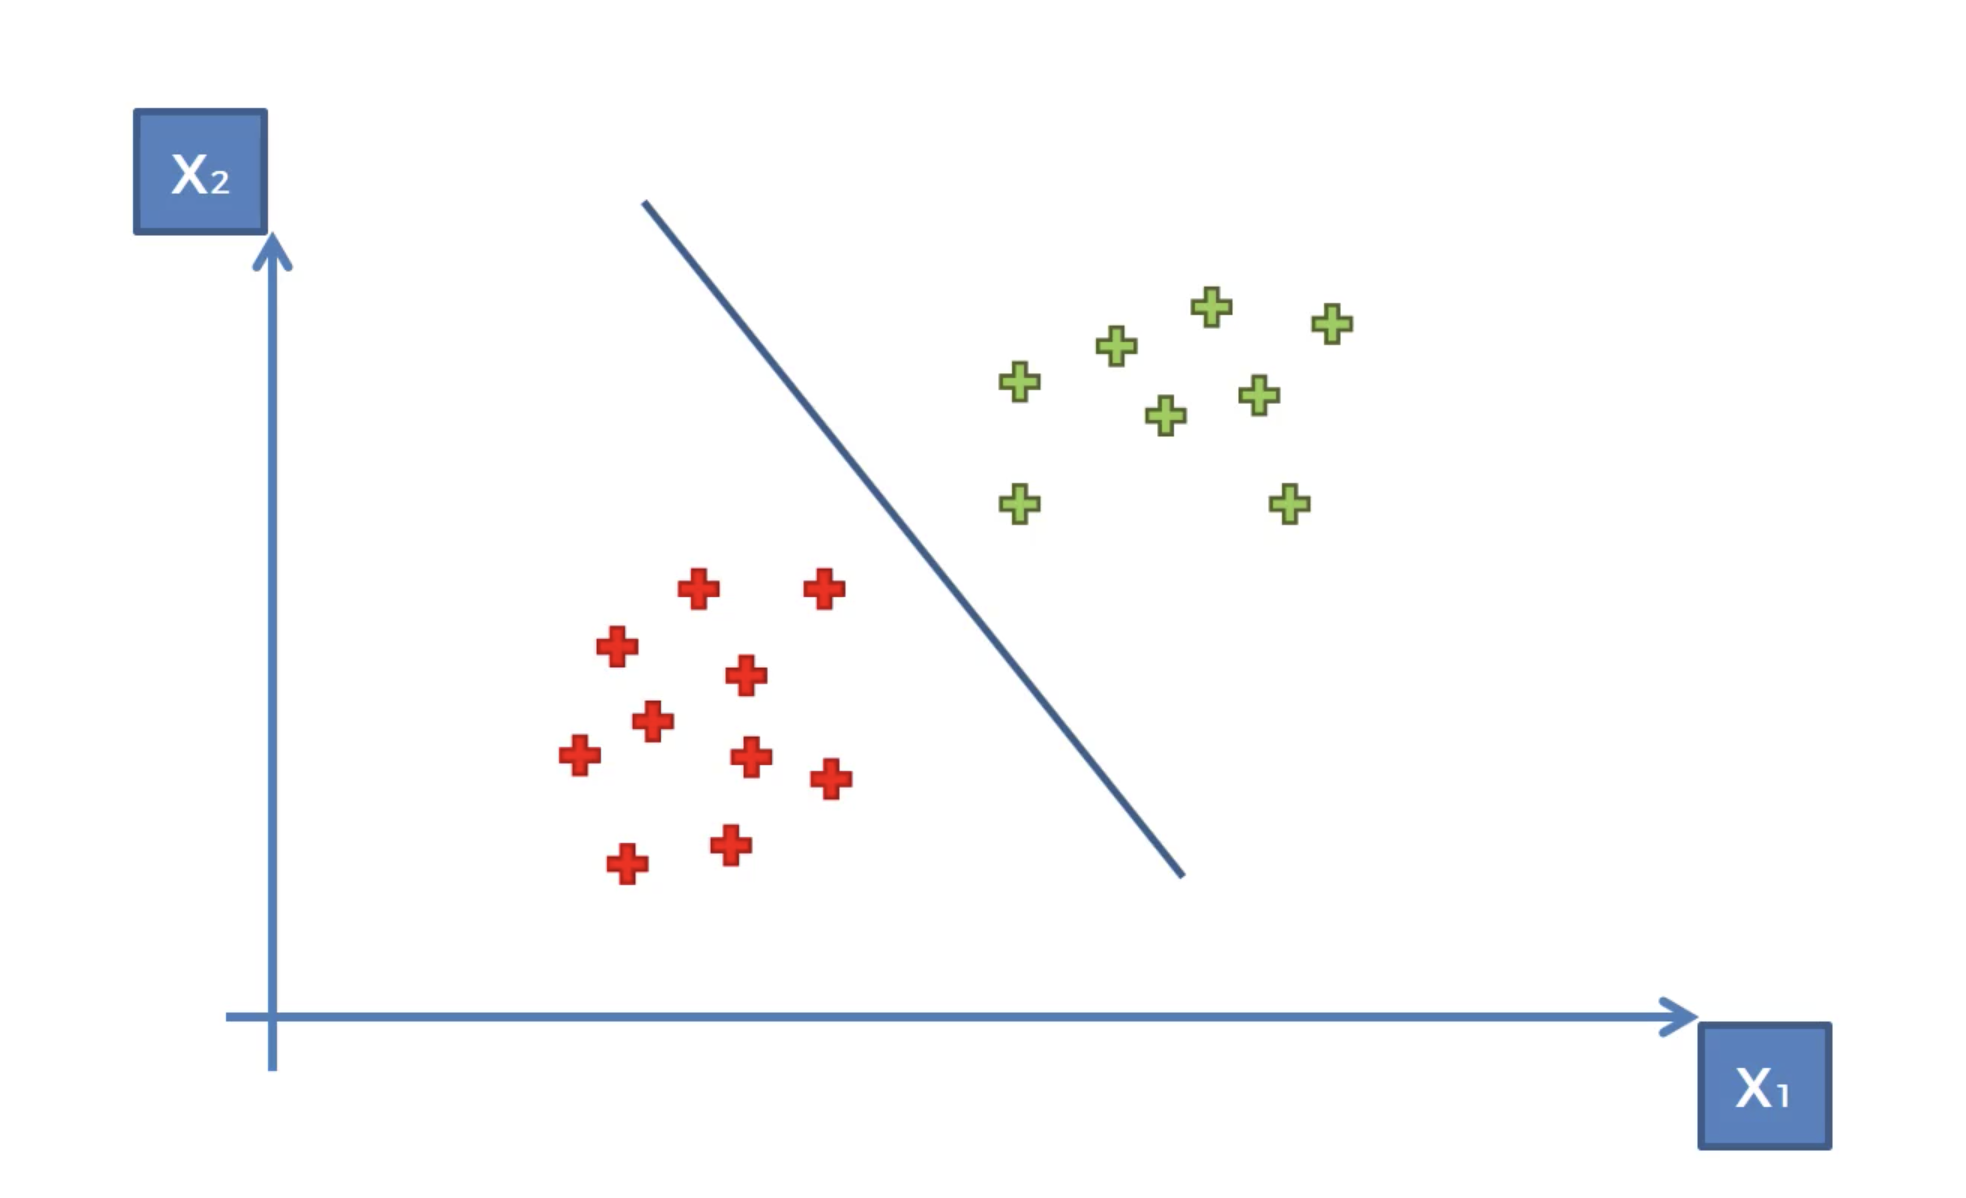
\includegraphics[width=0.85\linewidth ]{Figures/svm-1.png}


\end{frame}
%----------------------------------------------------------------------------%
\begin{frame}

\frametitle{Non Linearly Separable}

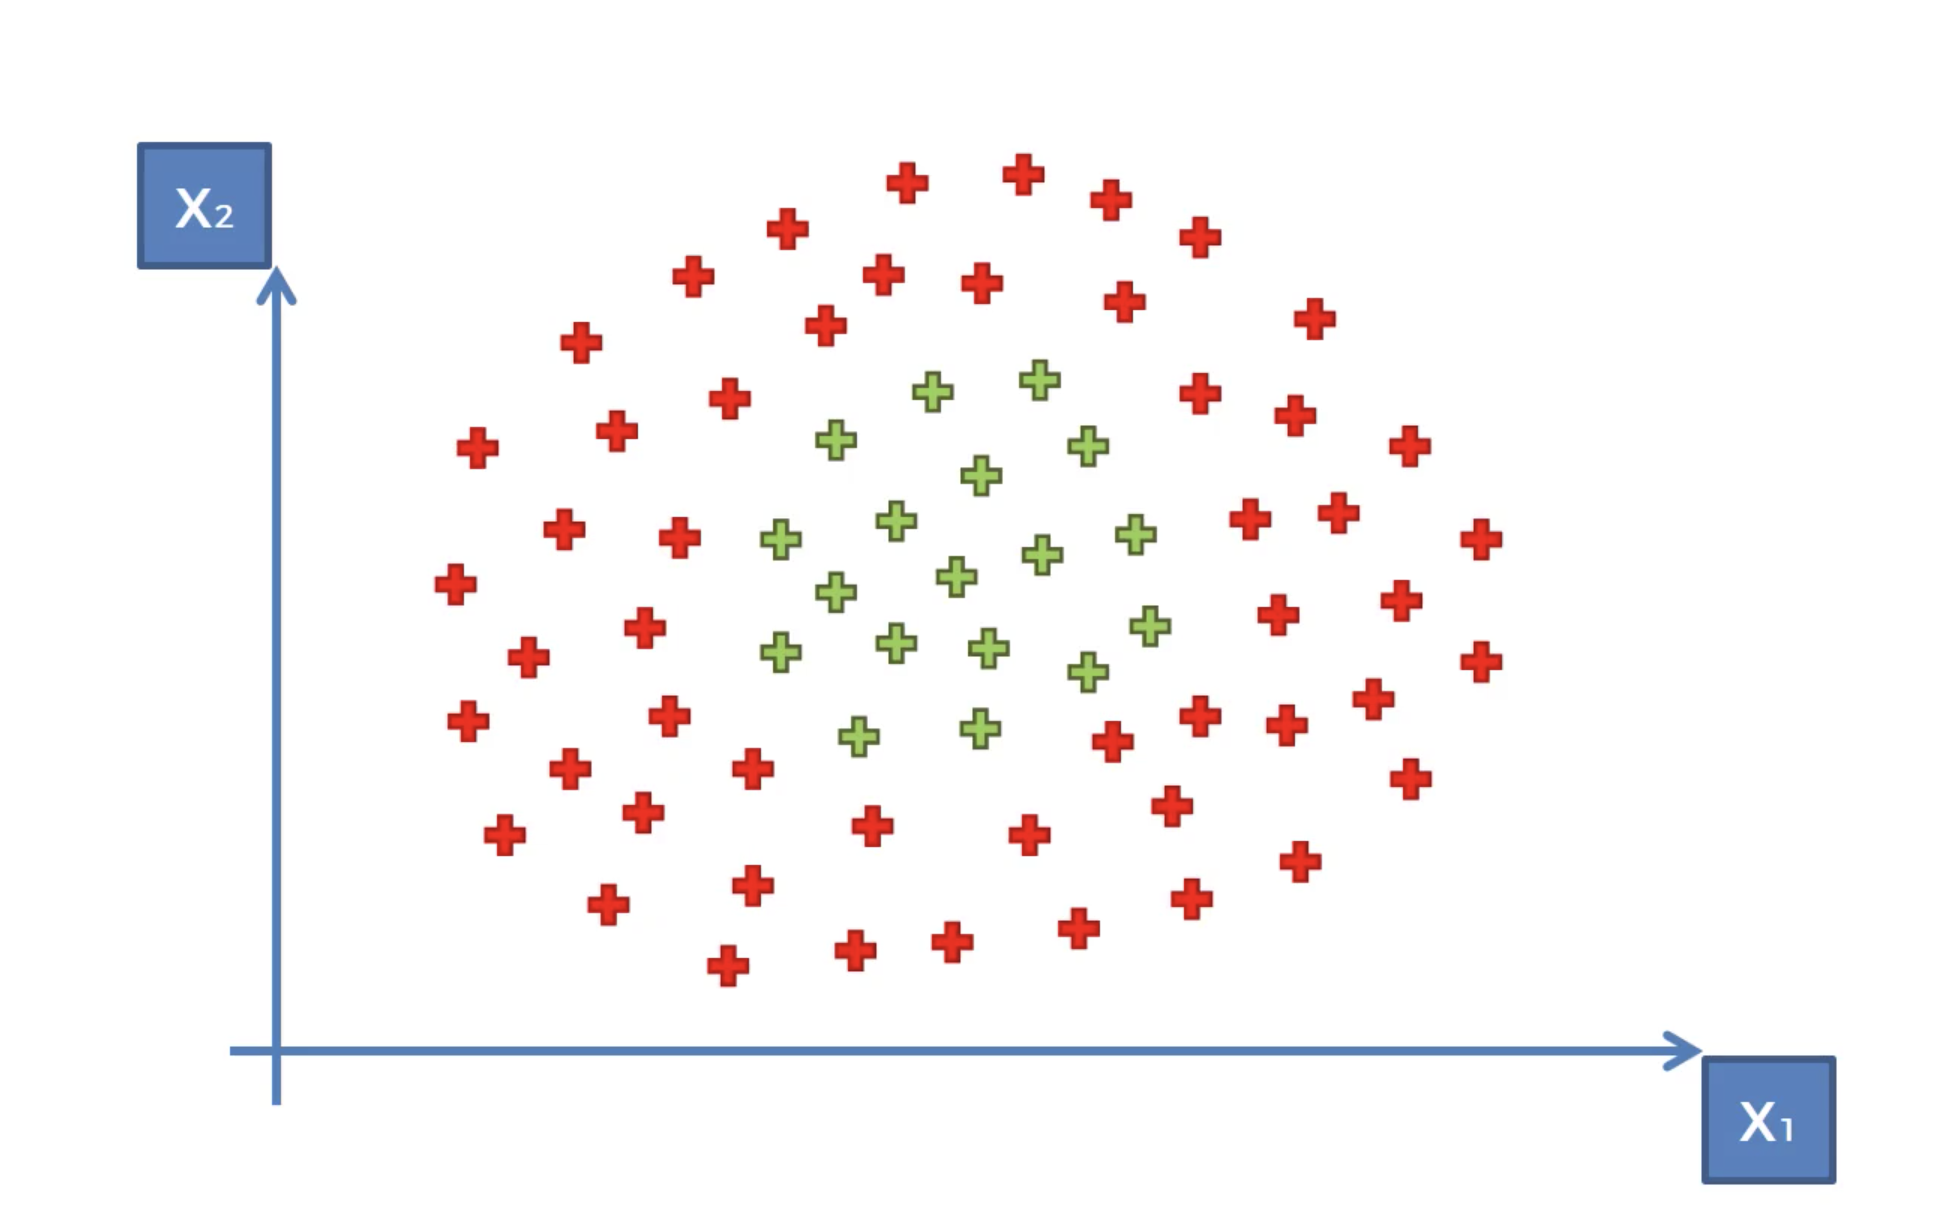
\includegraphics[width=0.85\linewidth ]{Figures/svm-2.png}


\end{frame}

%----------------------------------------------------------------------------%
 \begin{frame}

\frametitle{Non Linearly Separable}

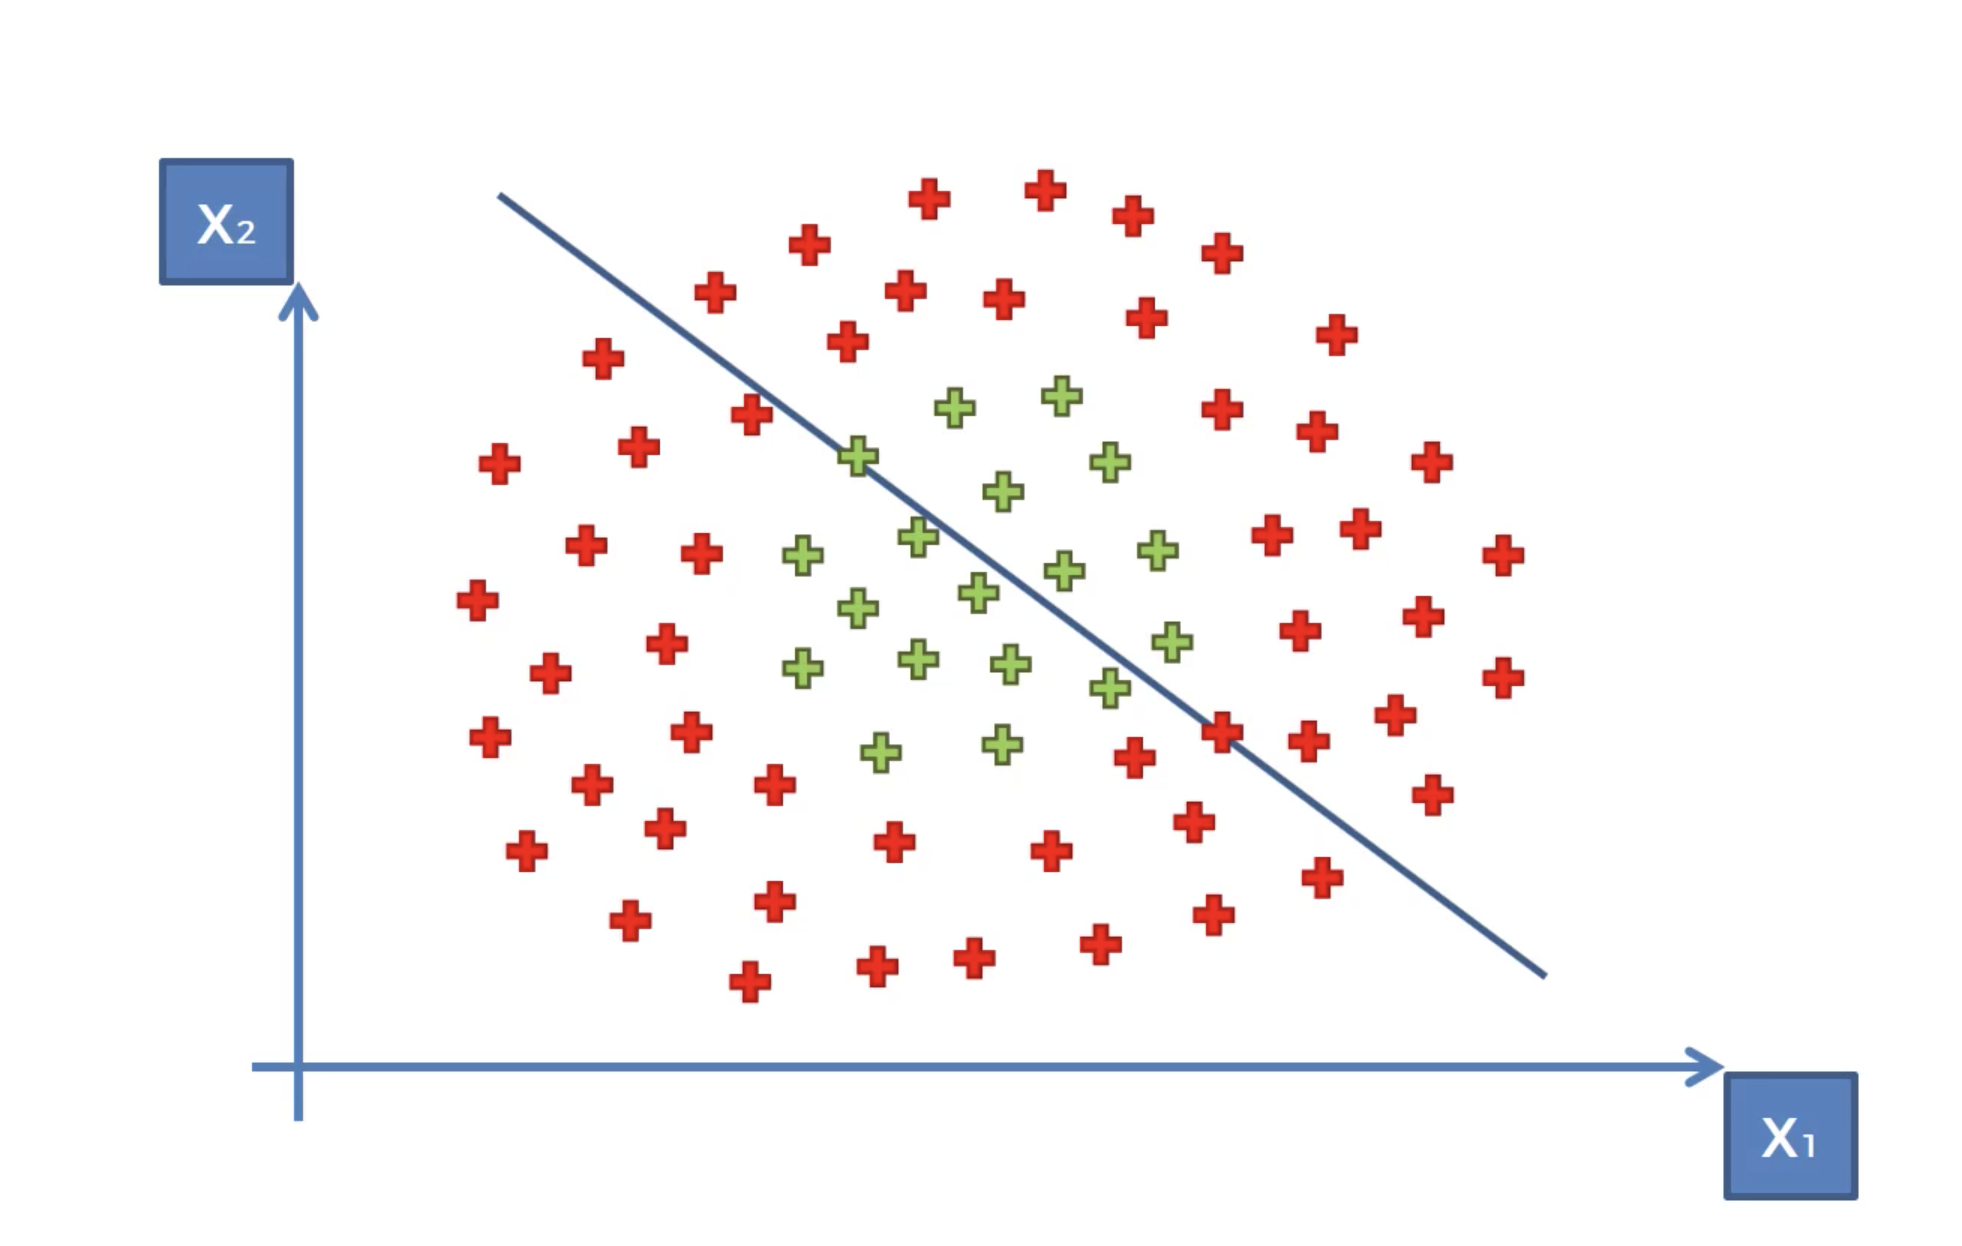
\includegraphics[width=0.85\linewidth ]{Figures/svm-3.png}


\end{frame}
%----------------------------------------------------------------------------%
 \begin{frame}

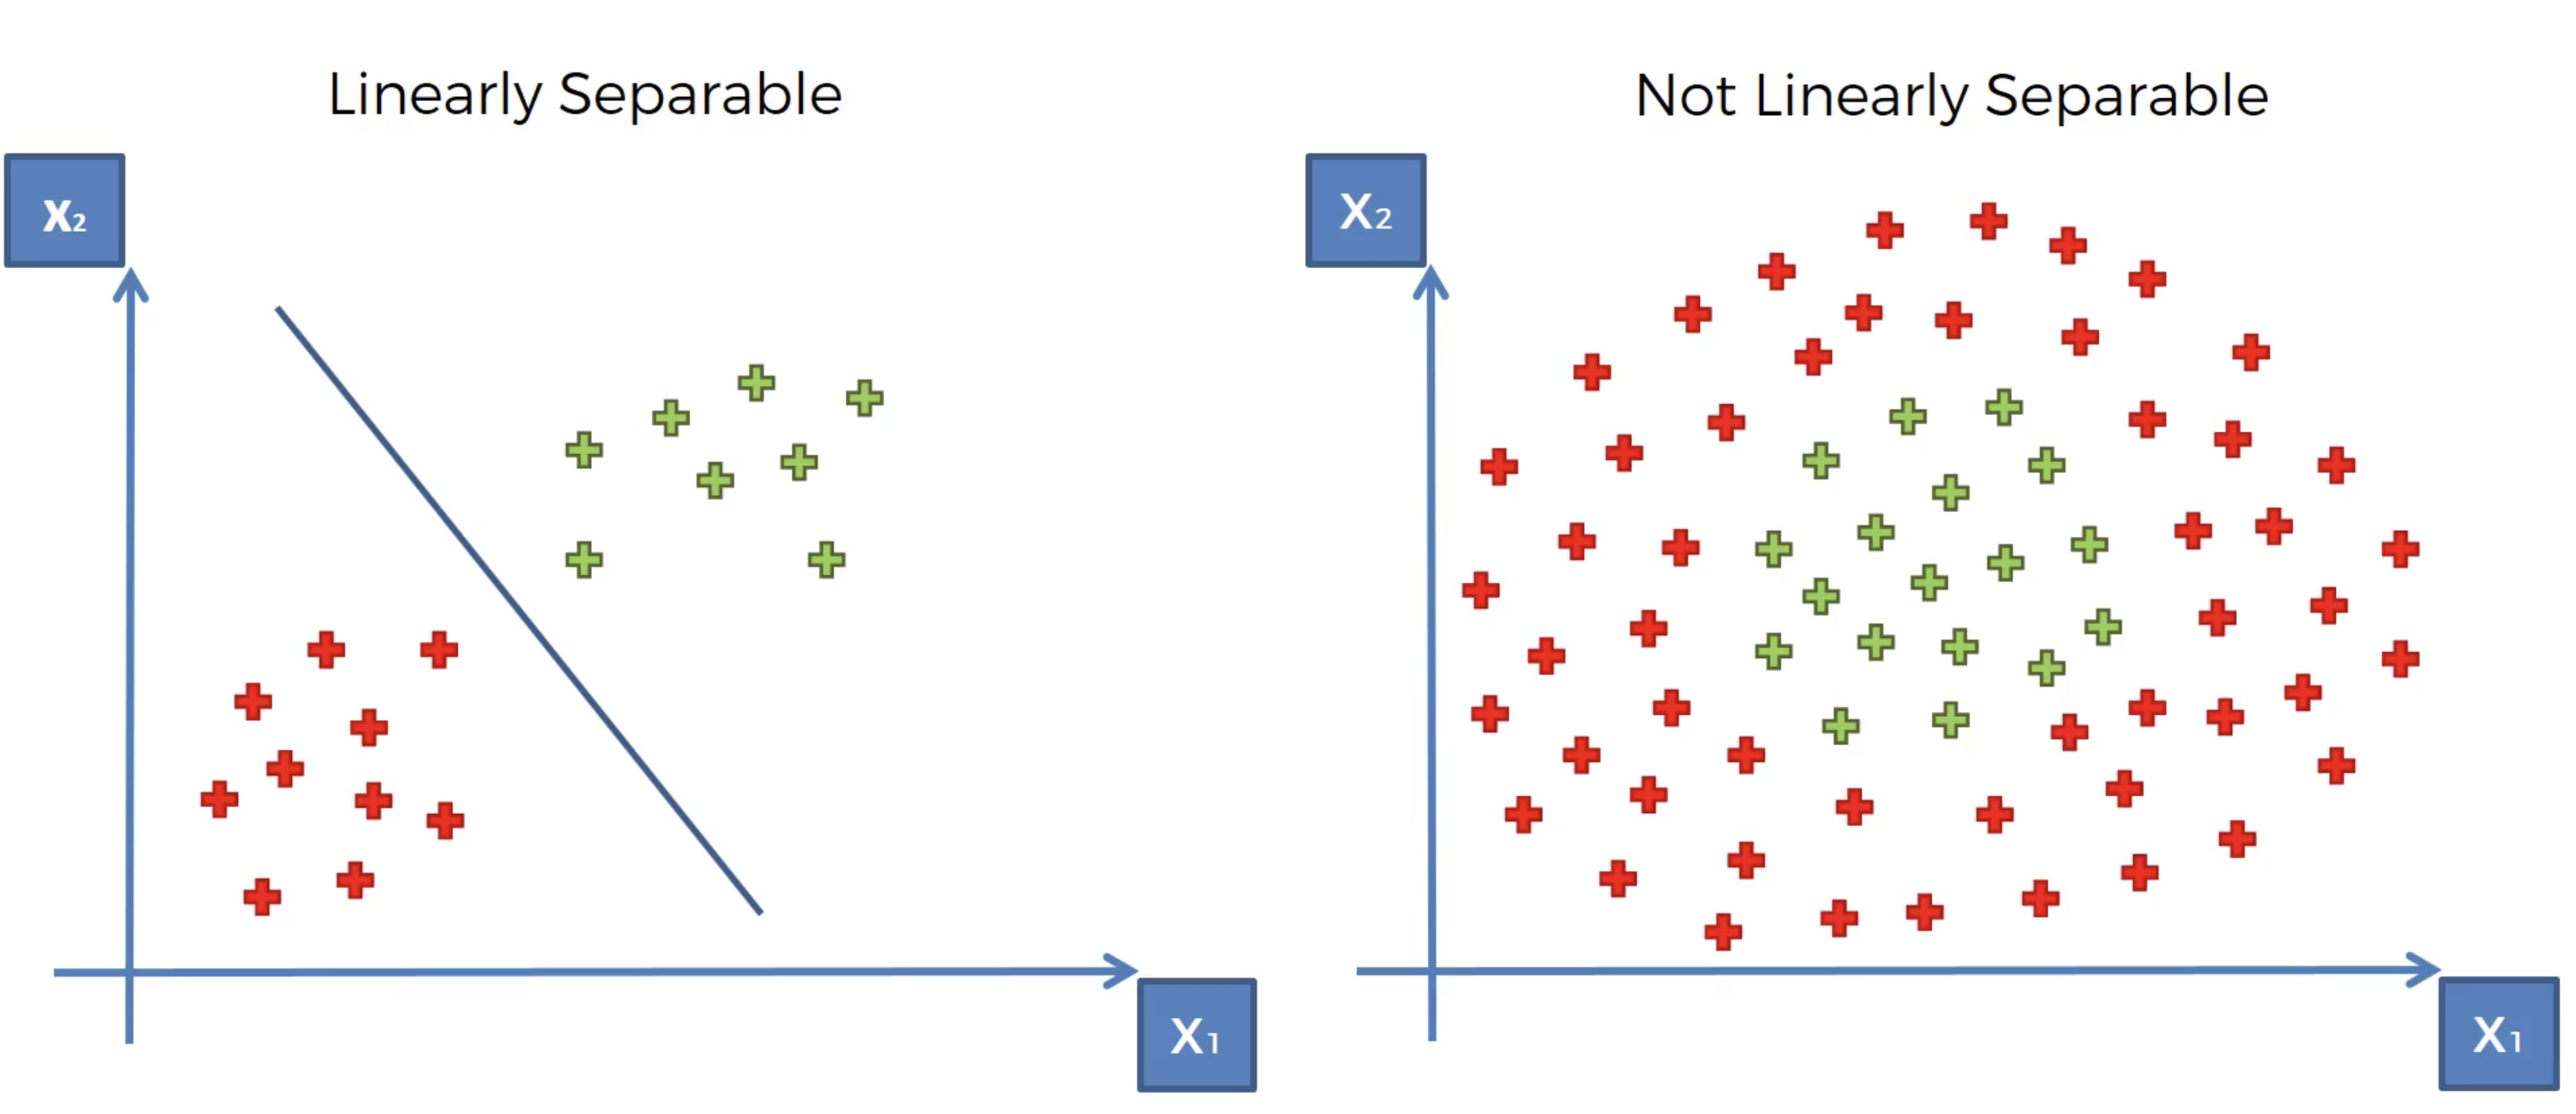
\includegraphics[width=0.85\linewidth ]{Figures/svm-4.png}


\end{frame}

\begin{frame}
\frametitle{Mapping to a higher dimension}
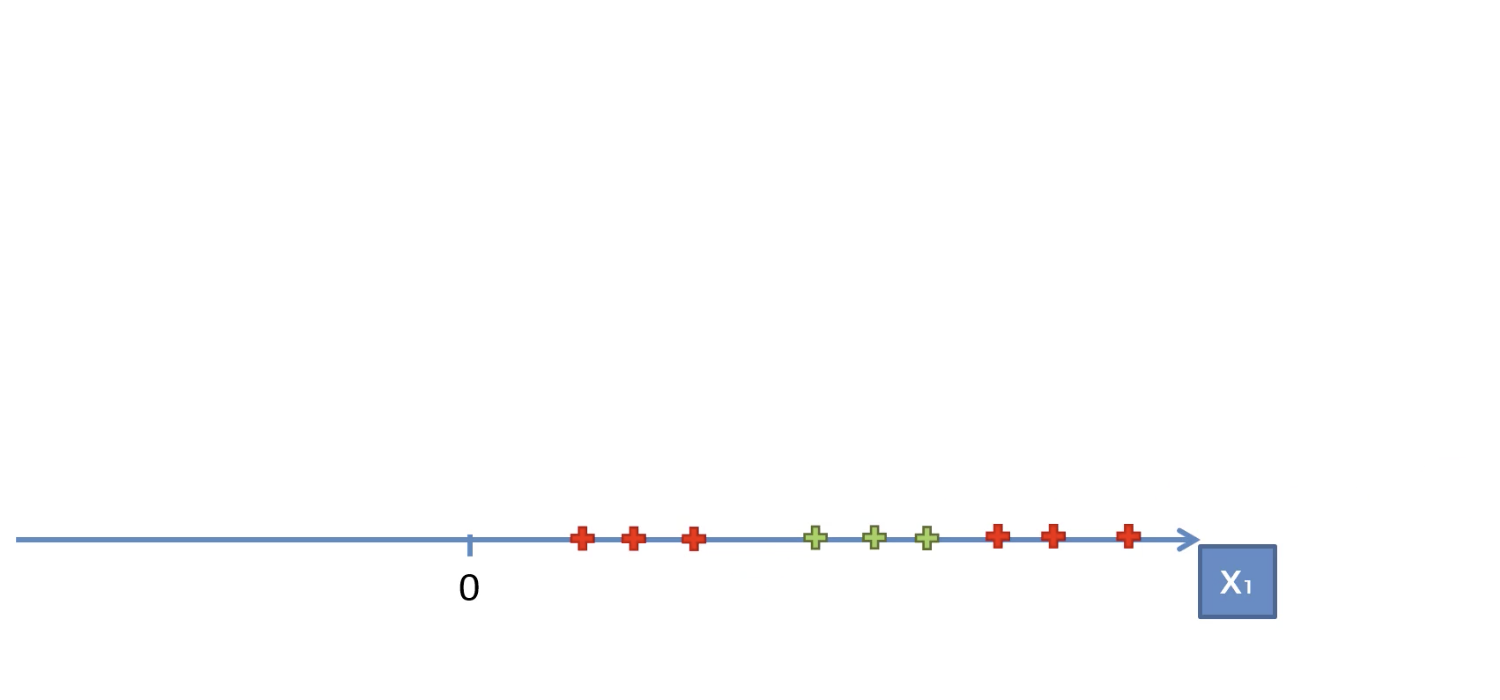
\includegraphics[width=0.85\linewidth ]{Figures/svm-f.png}


\end{frame}
%----------------------------------------------------------------------------%

%----------------------------------------------------------------------------%

%----------------------------------------------------------------------------%


\begin{frame}
\frametitle{Mapping to a higher dimension}
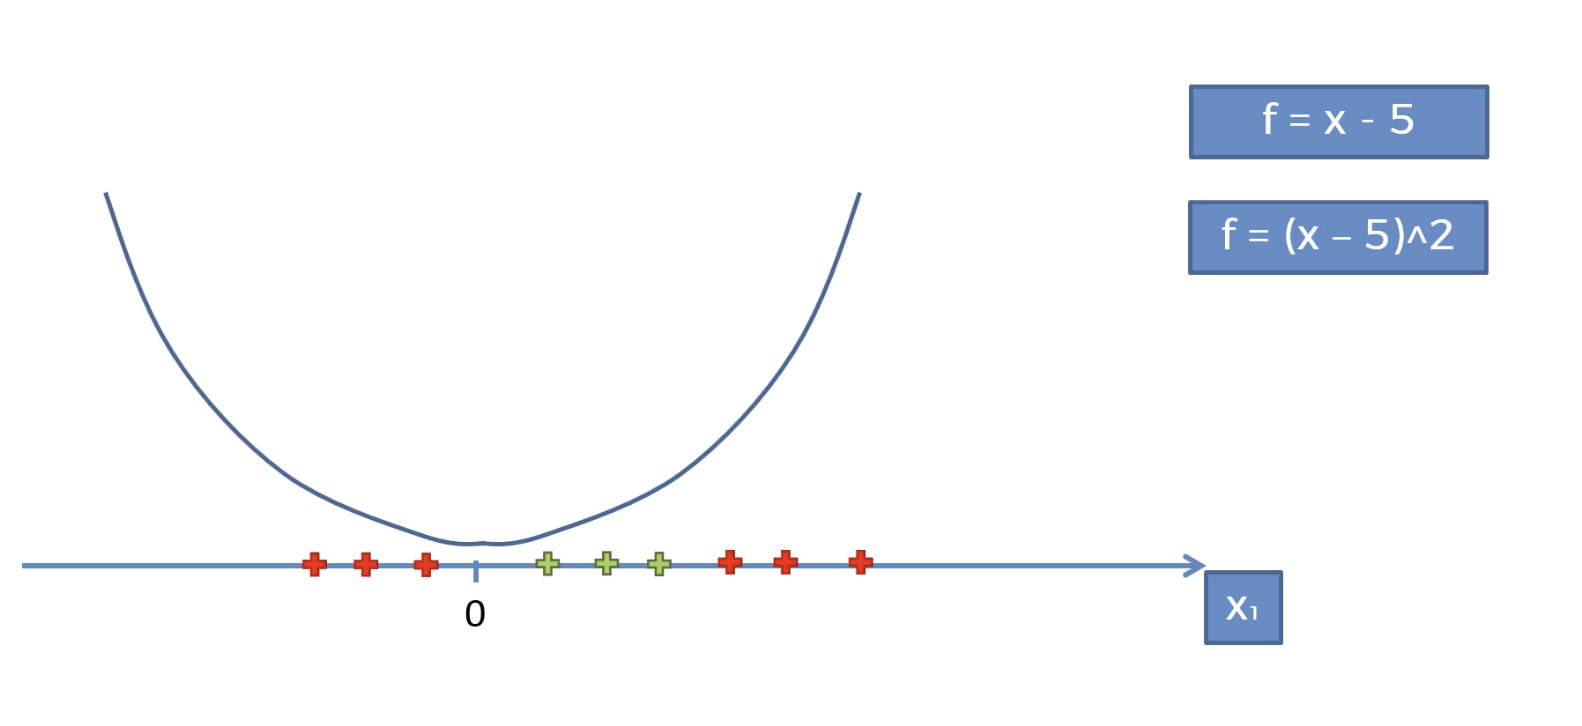
\includegraphics[width=0.85\linewidth ]{Figures/svm-f3.png}


\end{frame}
%----------------------------------------------------------------------------%

 
\begin{frame}
\frametitle{Mapping to a higher dimension}
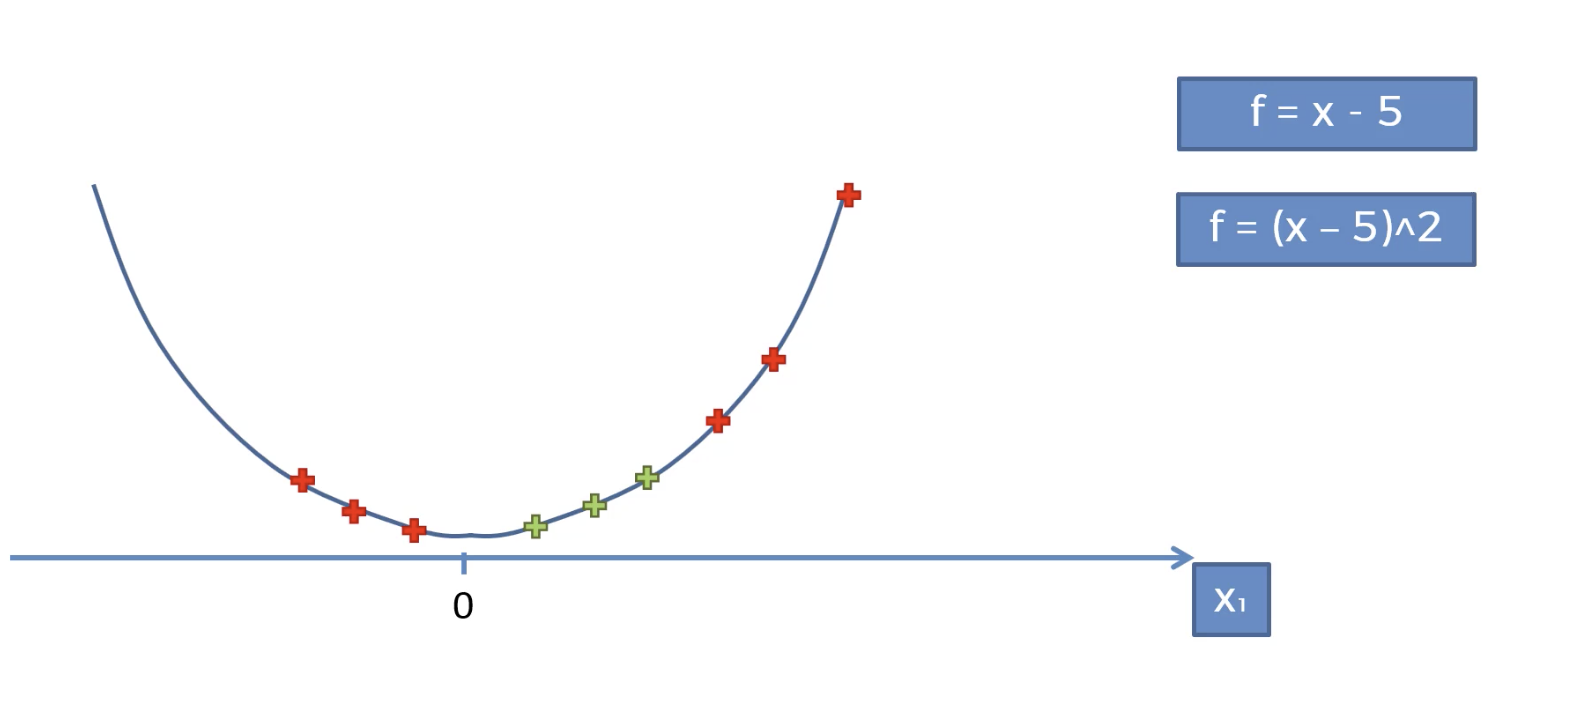
\includegraphics[width=0.85\linewidth ]{Figures/svm-f4.png}


\end{frame}
%----------------------------------------------------------------------------%
%----------------------------------------------------------------------------%

\begin{frame}
\frametitle{Mapping to a higher dimension}
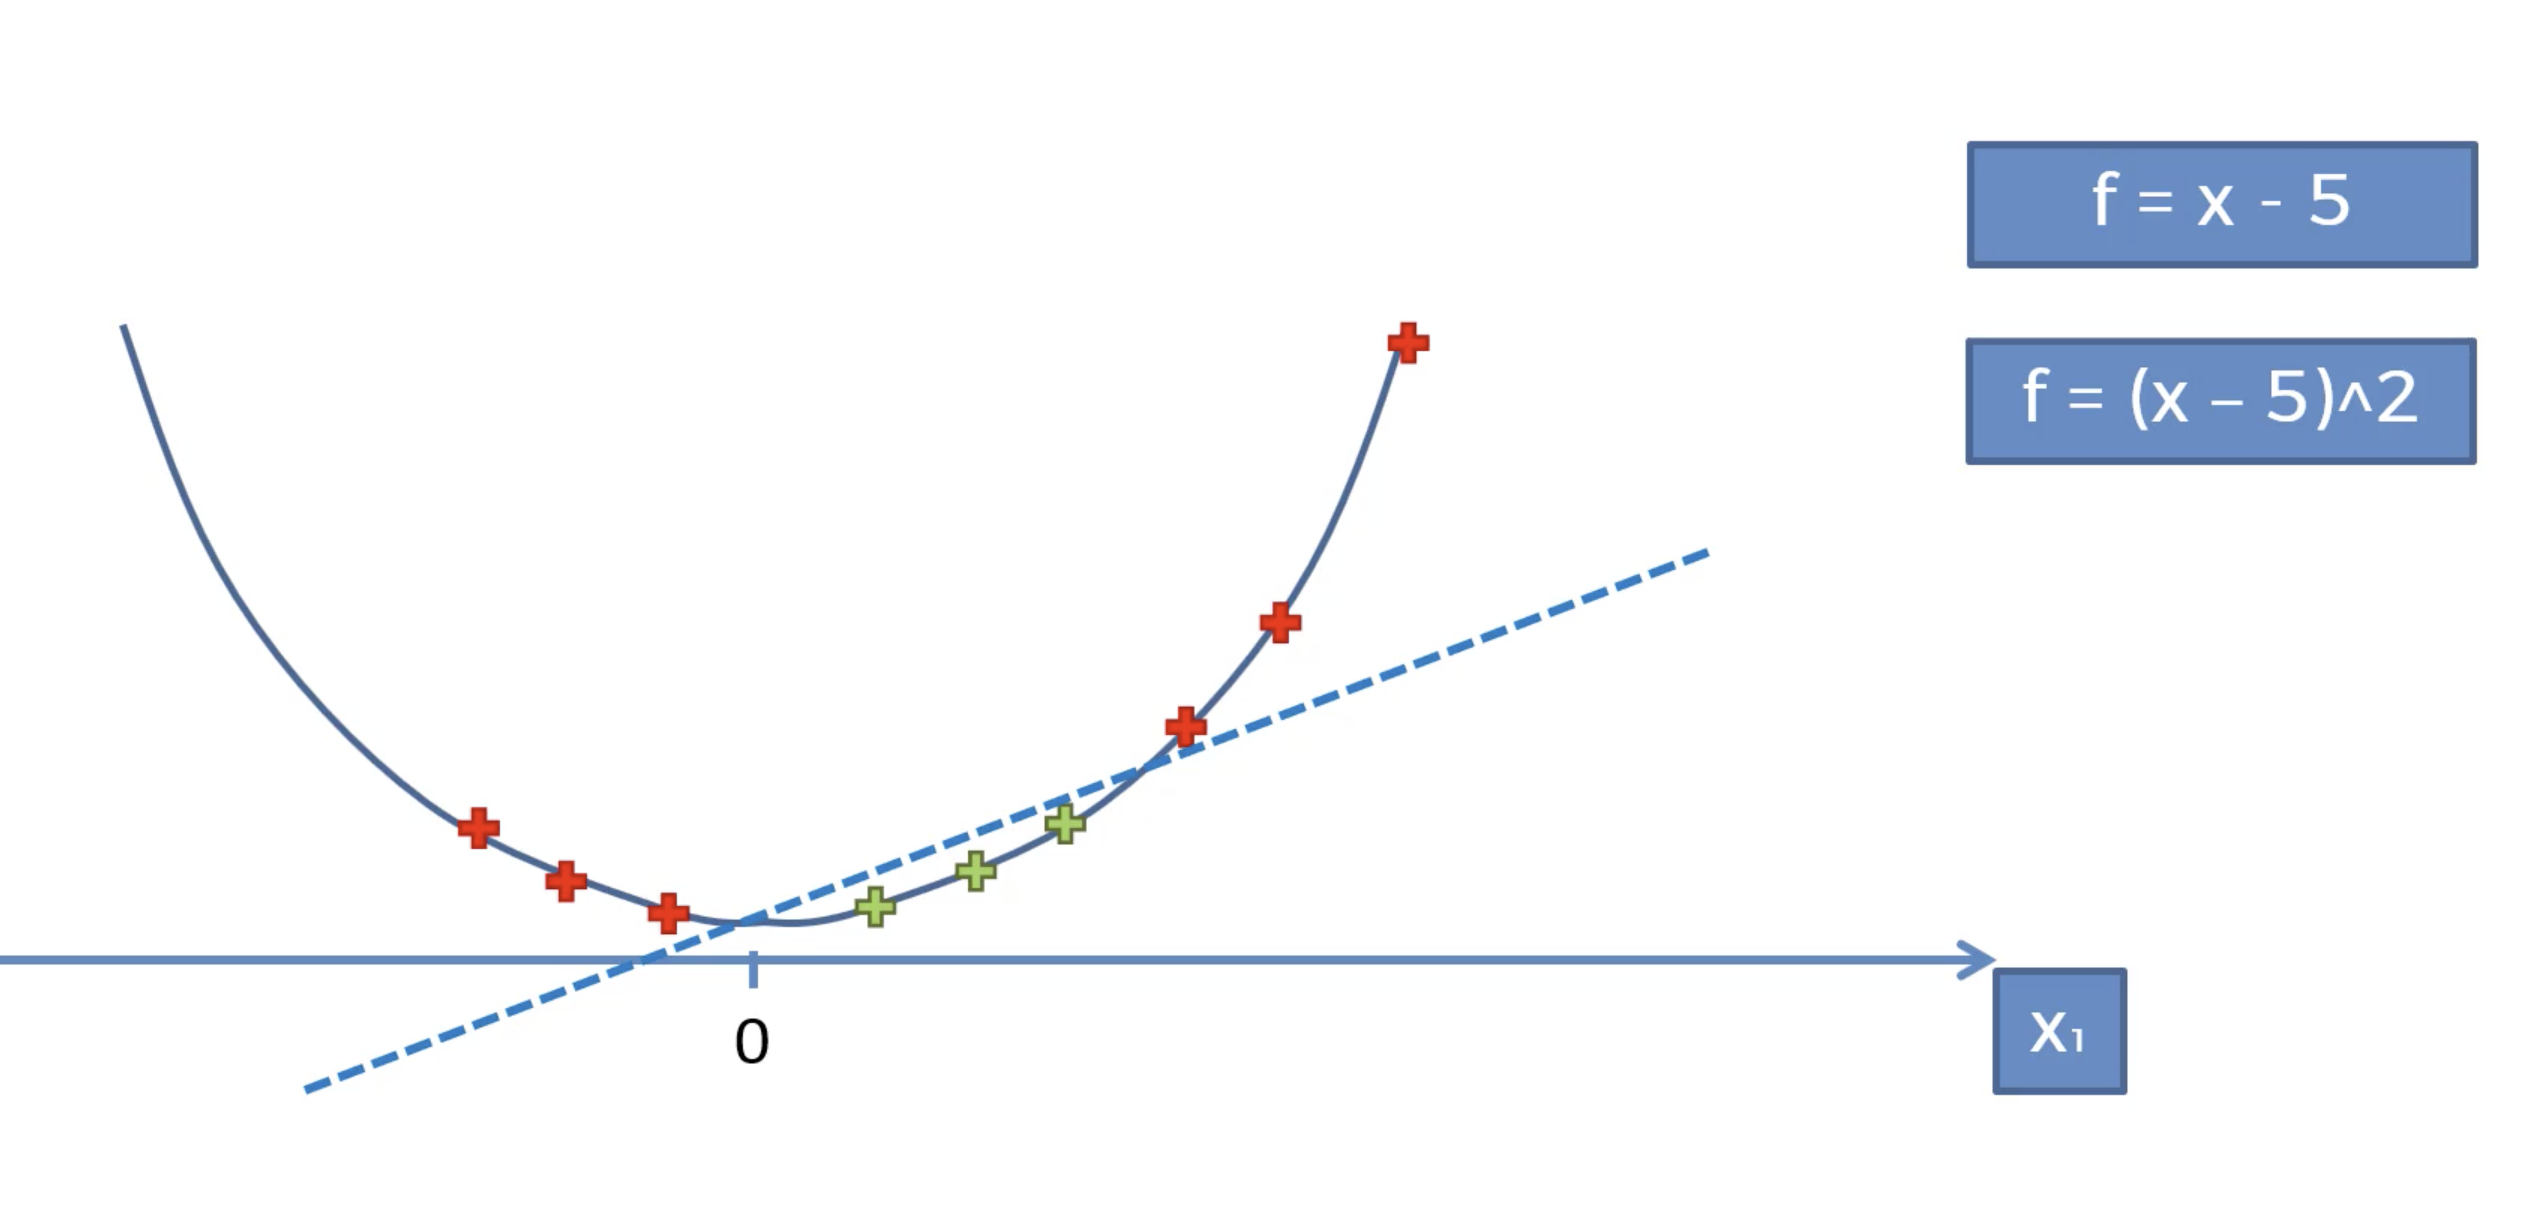
\includegraphics[width=0.85\linewidth ]{Figures/svm-f5.png}


\end{frame}
%----------------------------------------------------------------------------%
\begin{frame}
\frametitle{Mapping to a higher dimension}
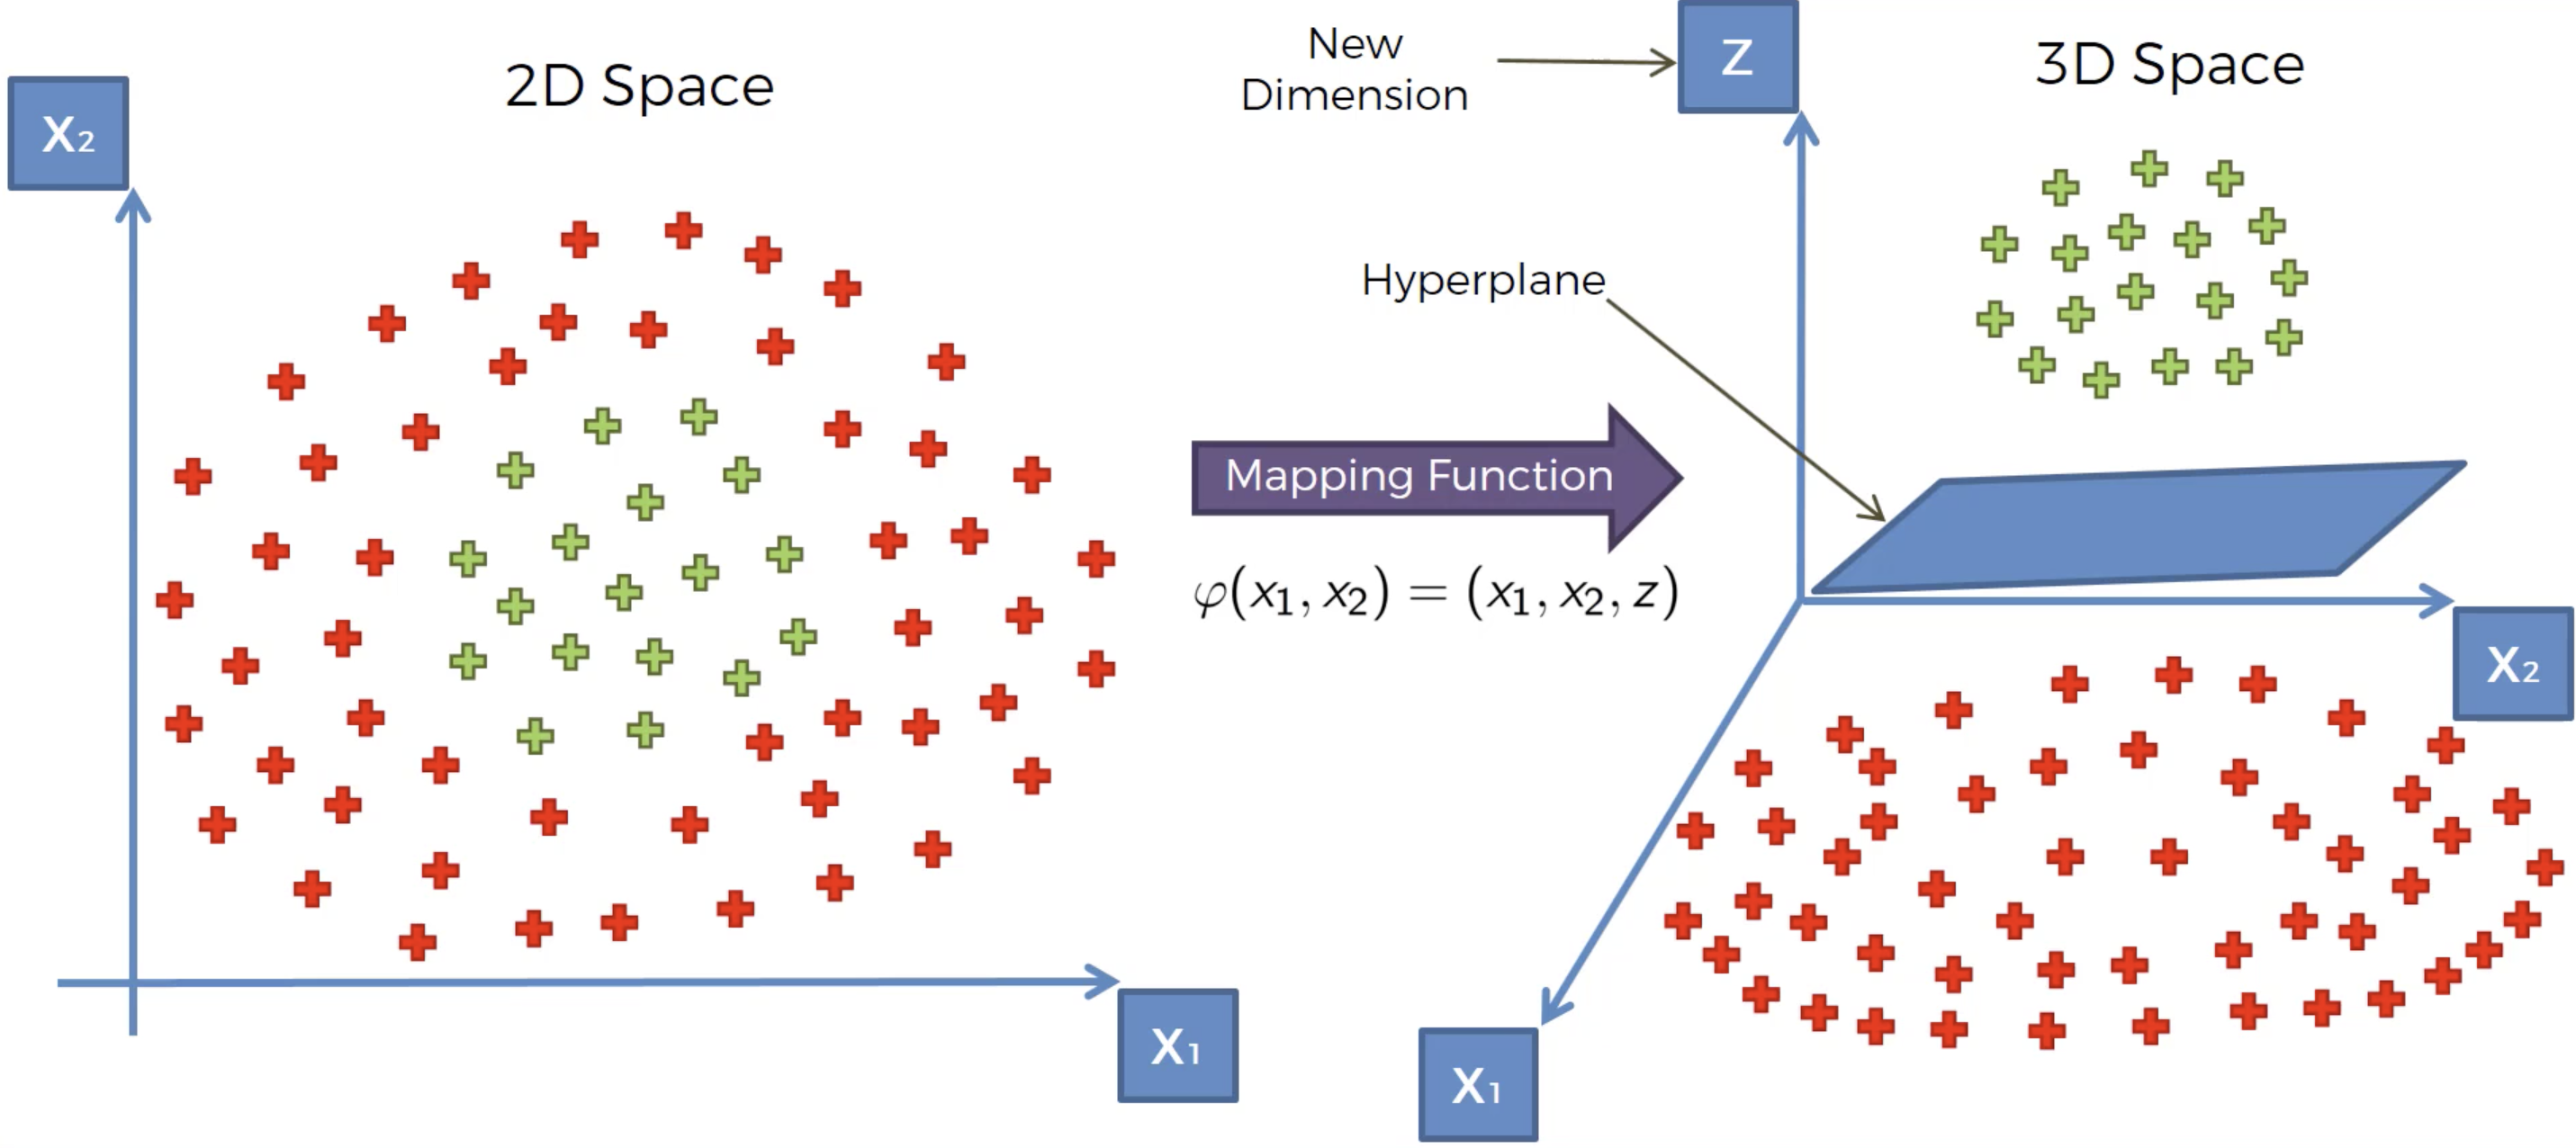
\includegraphics[width=0.85\linewidth ]{Figures/svm-f6.png}


\end{frame}

%----------------------------------------------------------------------------%
\begin{frame}
\frametitle{The Kernel Trick: RBF-Kernel}
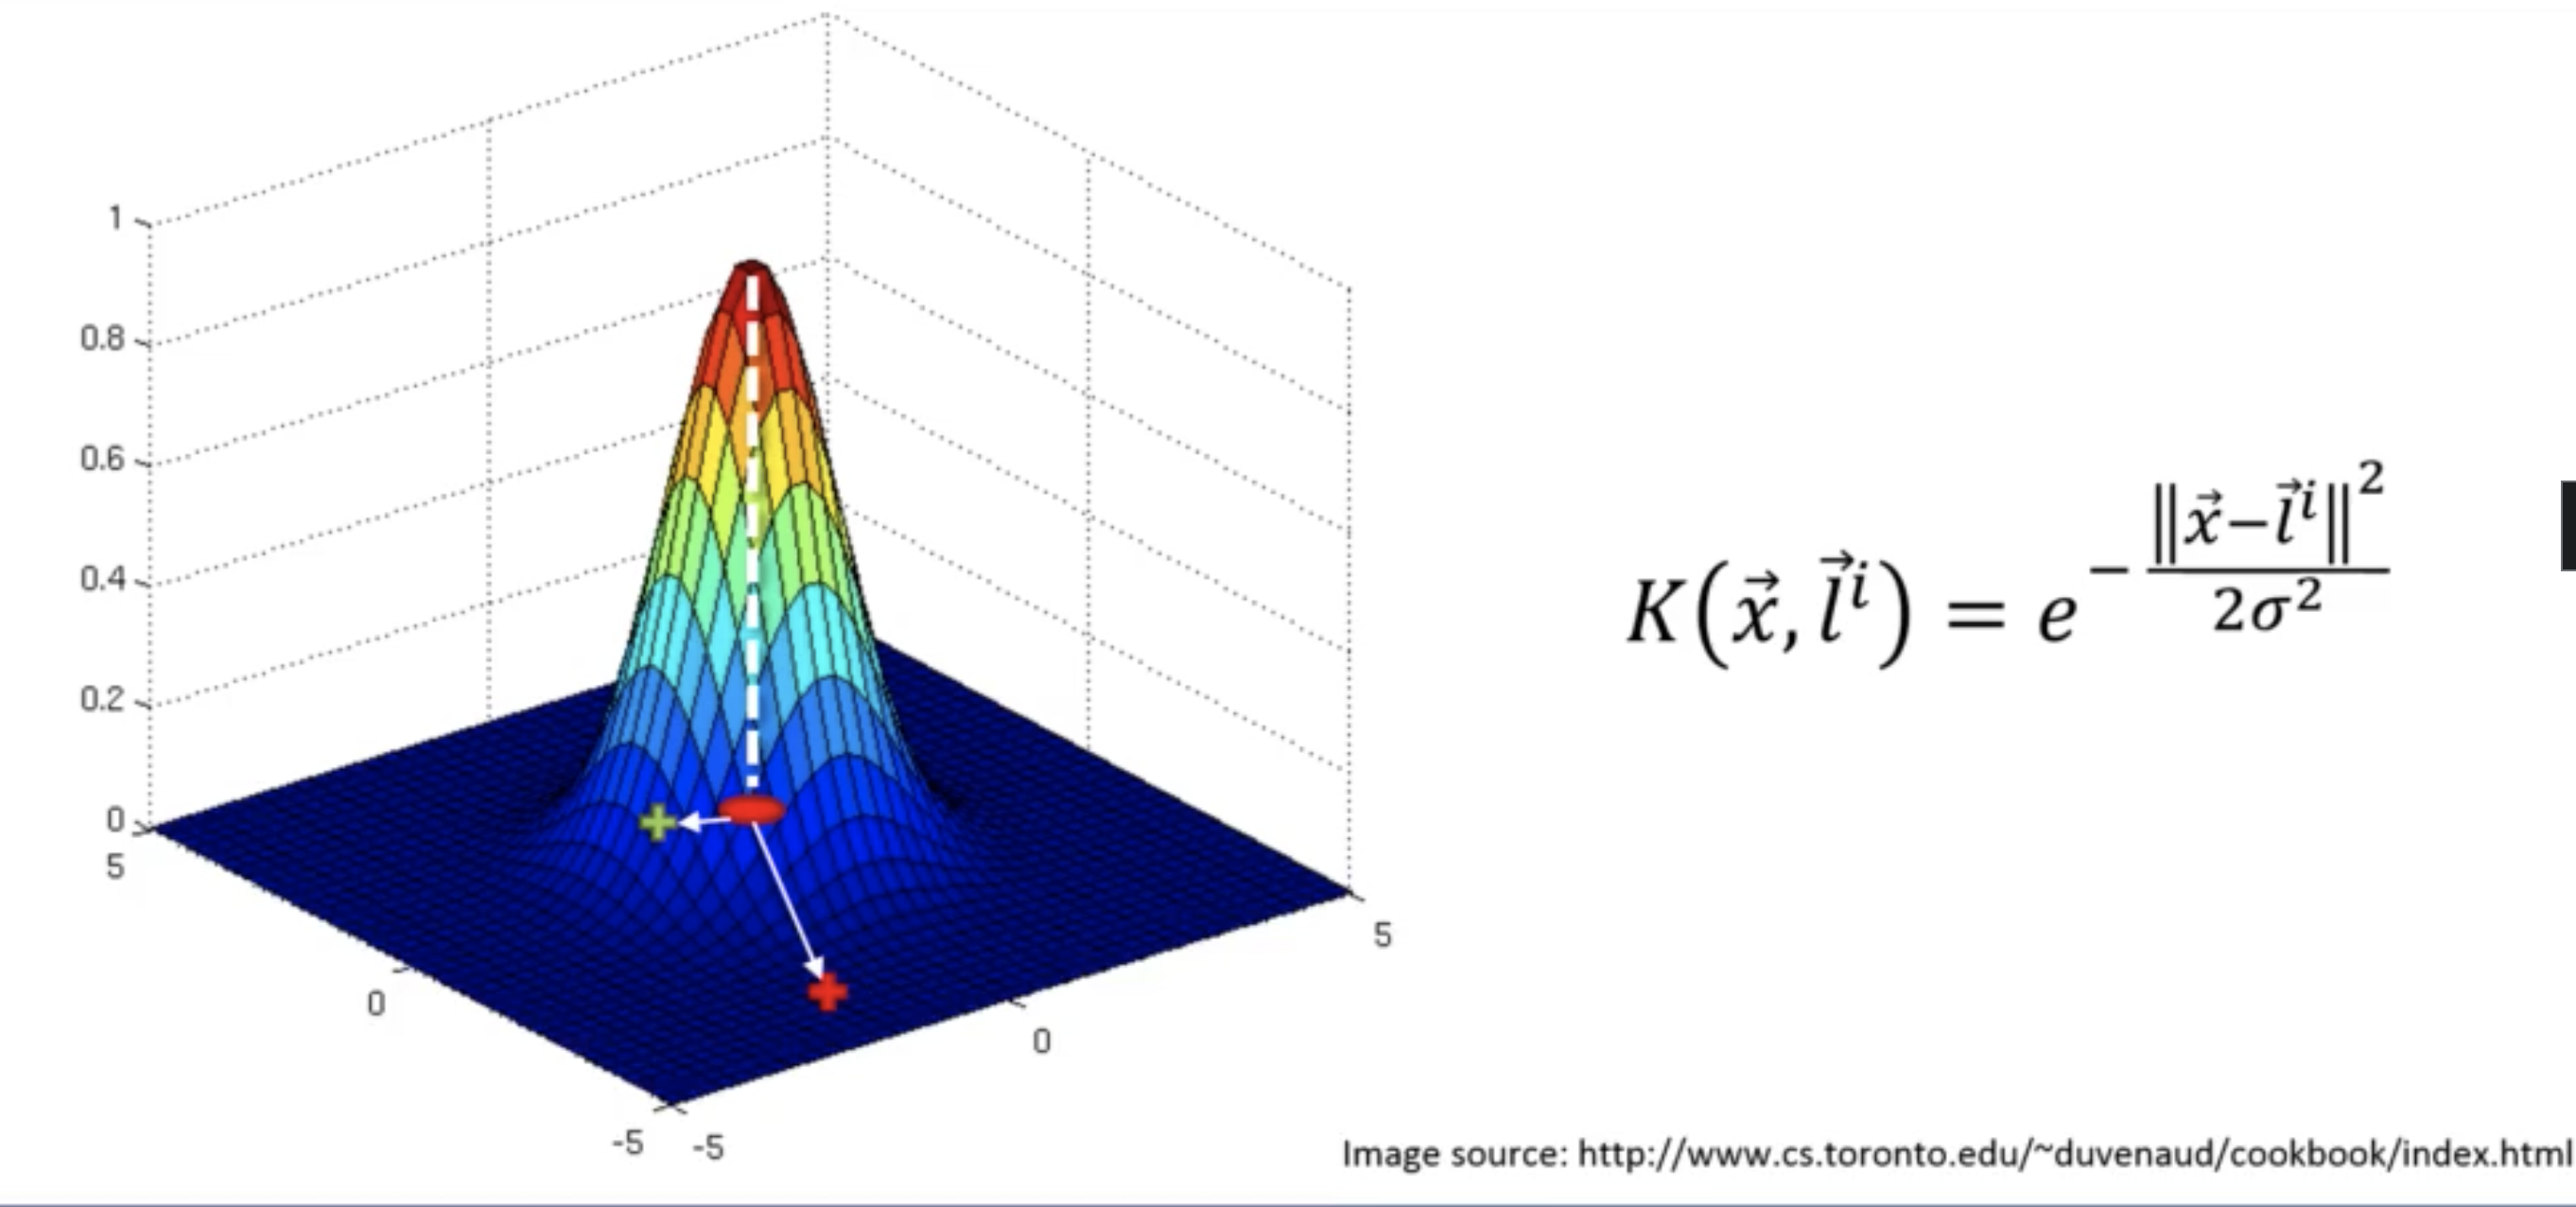
\includegraphics[width=0.85\linewidth ]{Figures/svm-rbf.png}


\end{frame}

\begin{frame}
\frametitle{RBF-Kernel}
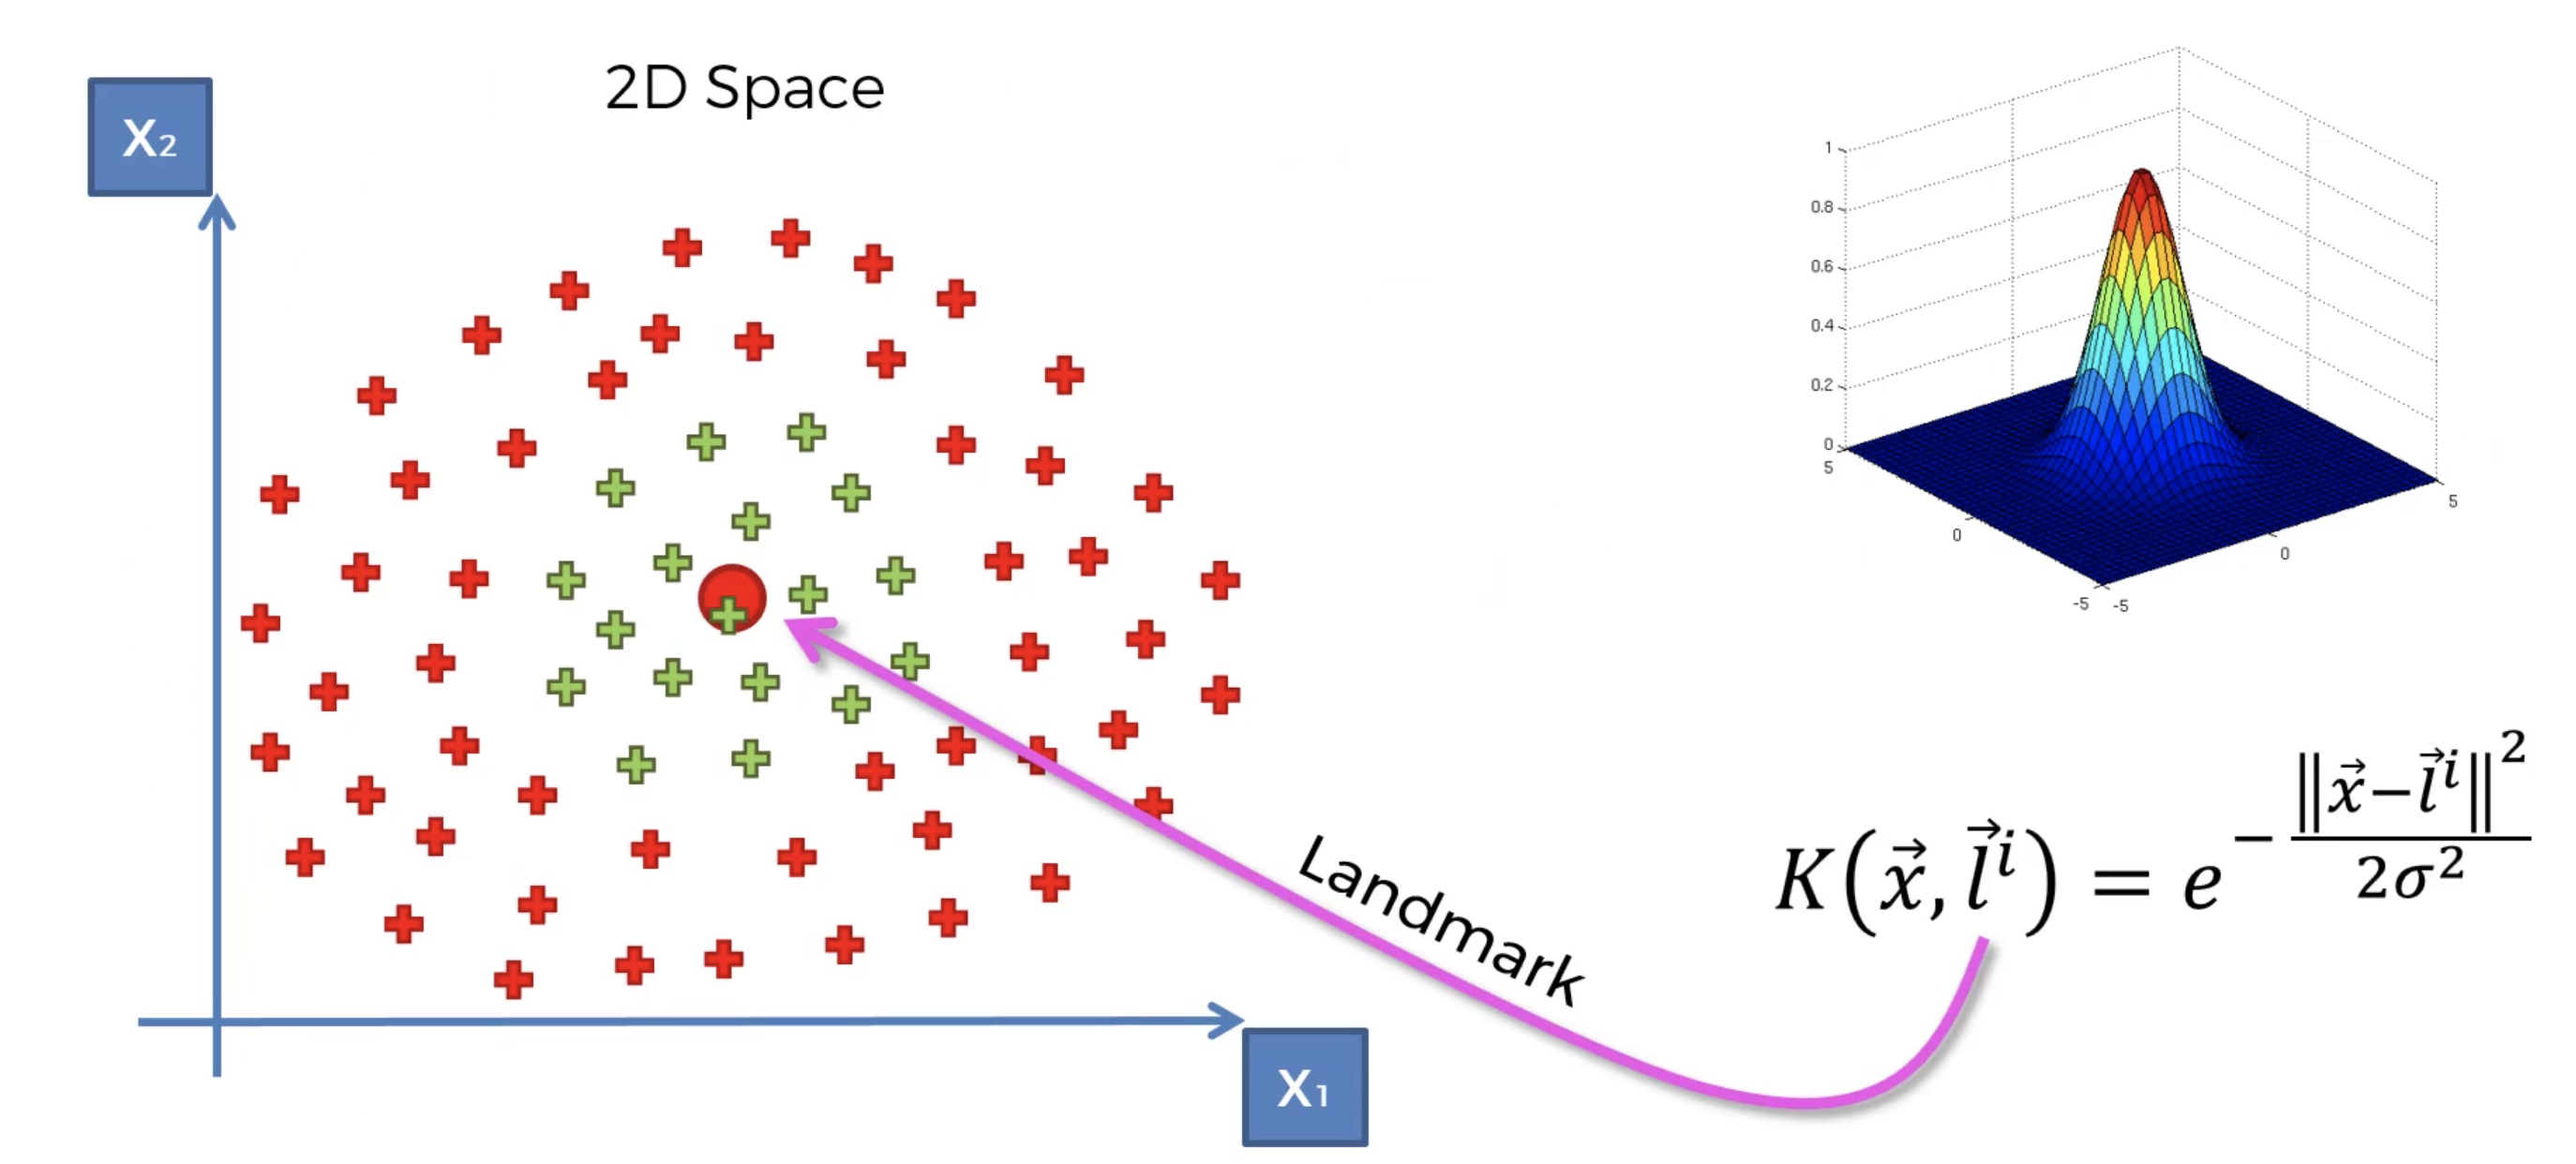
\includegraphics[width=0.85\linewidth ]{Figures/svm-rbf2.png}

\end{frame}

\begin{frame}
\frametitle{RBF-Kernel}
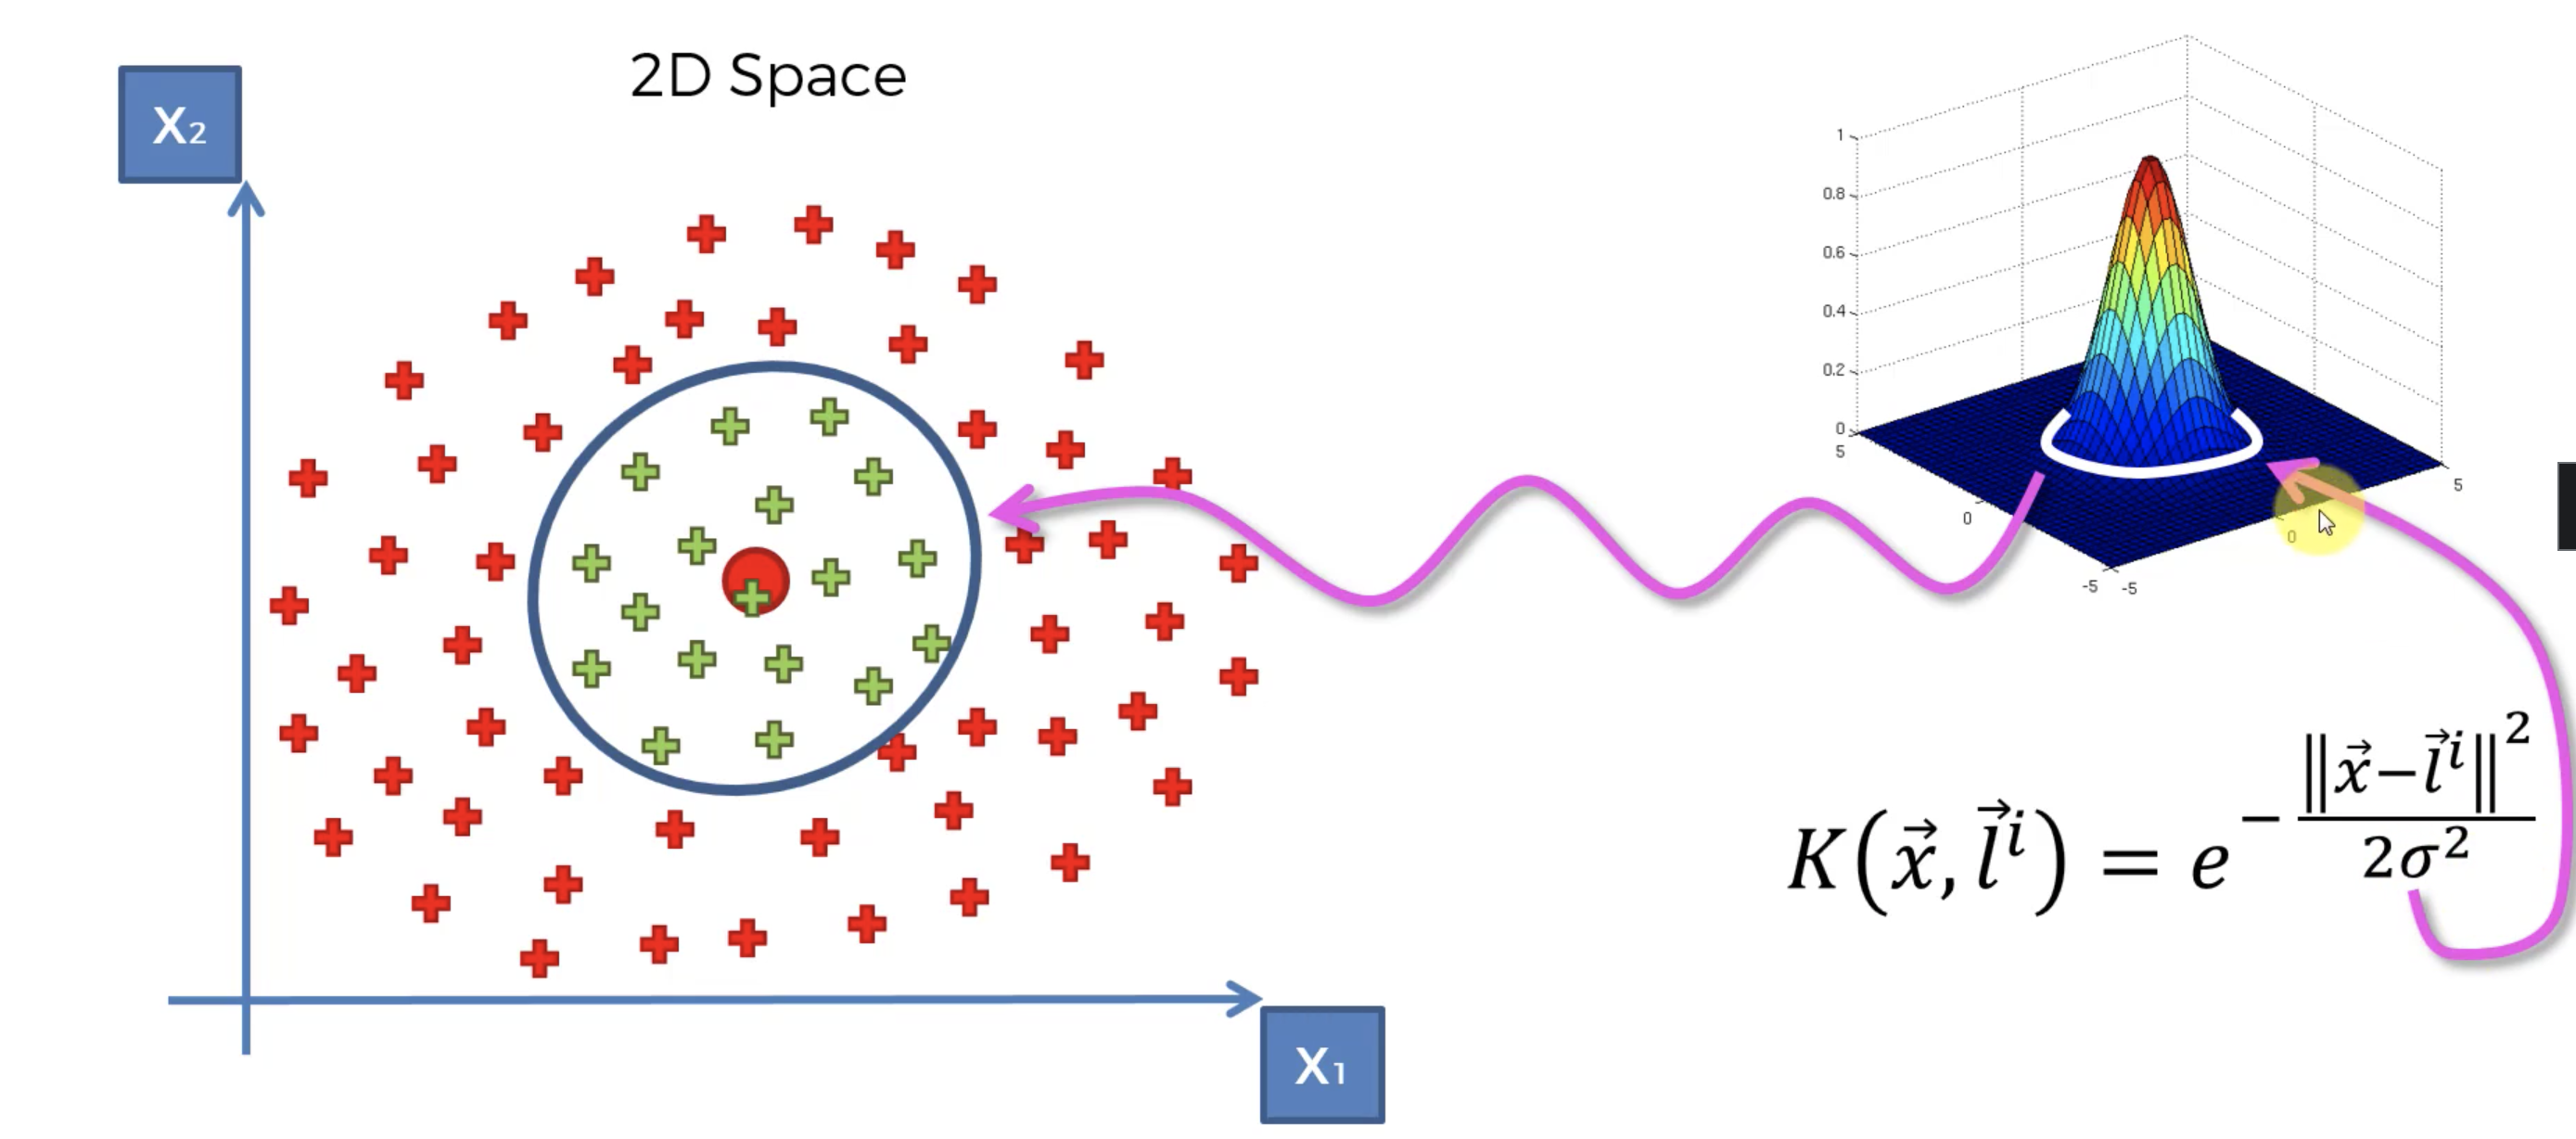
\includegraphics[width=0.85\linewidth ]{Figures/svm-rbf3.png}

\end{frame}


\begin{frame}
\frametitle{RBF-Kernel}
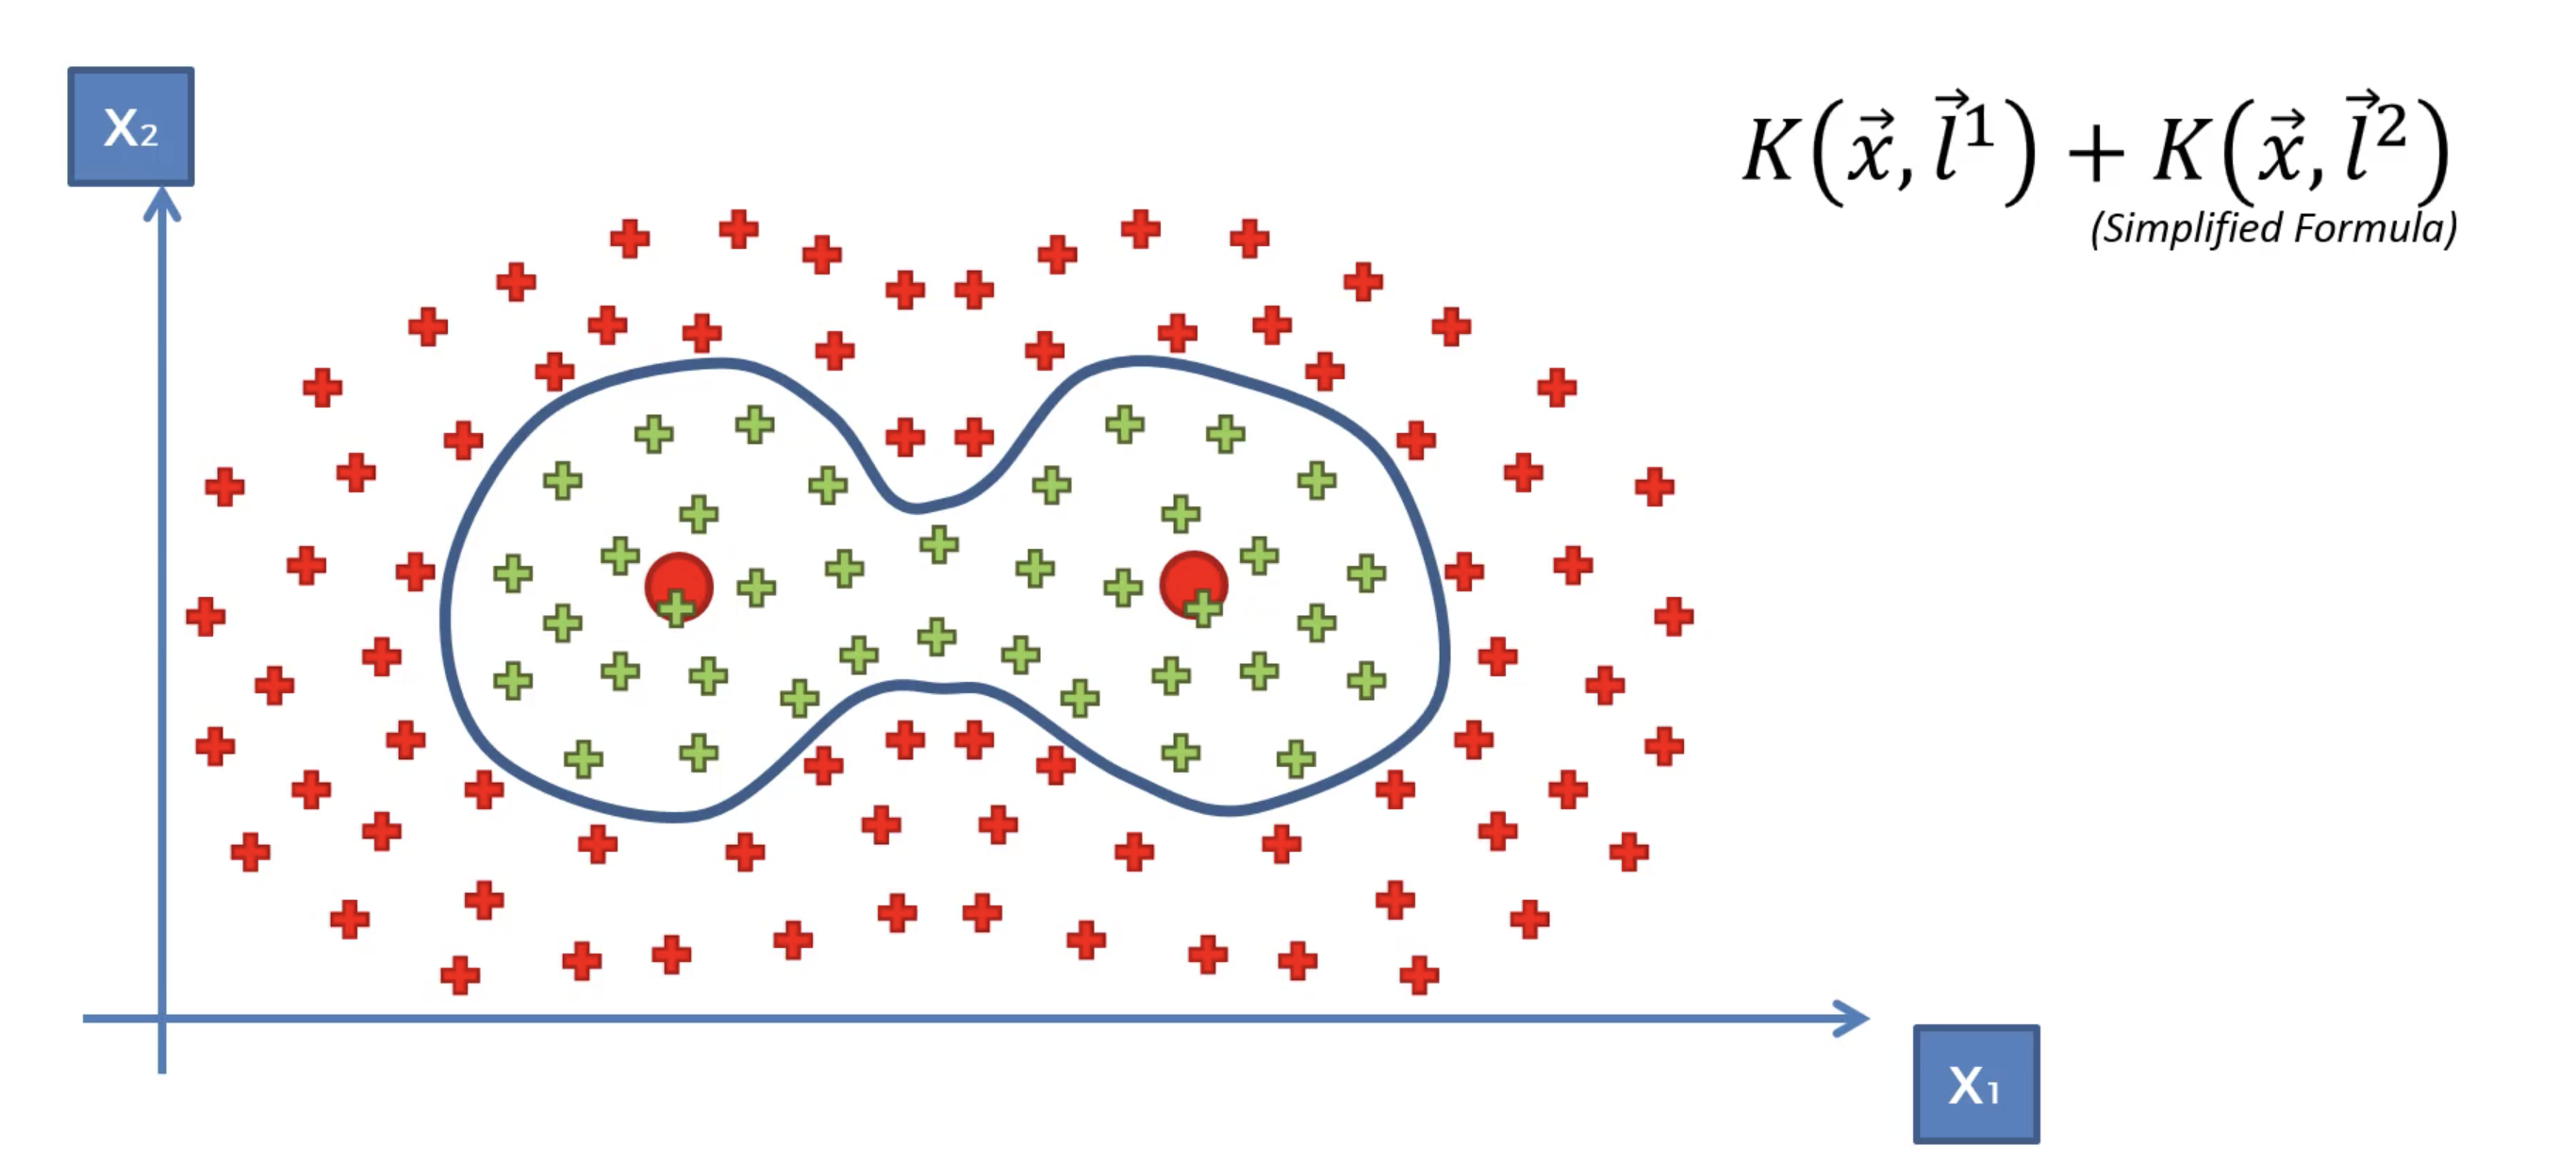
\includegraphics[width=0.85\linewidth ]{Figures/svm-rbf4.png}

\end{frame}

\begin{frame}
\frametitle{Most Common Kernels}
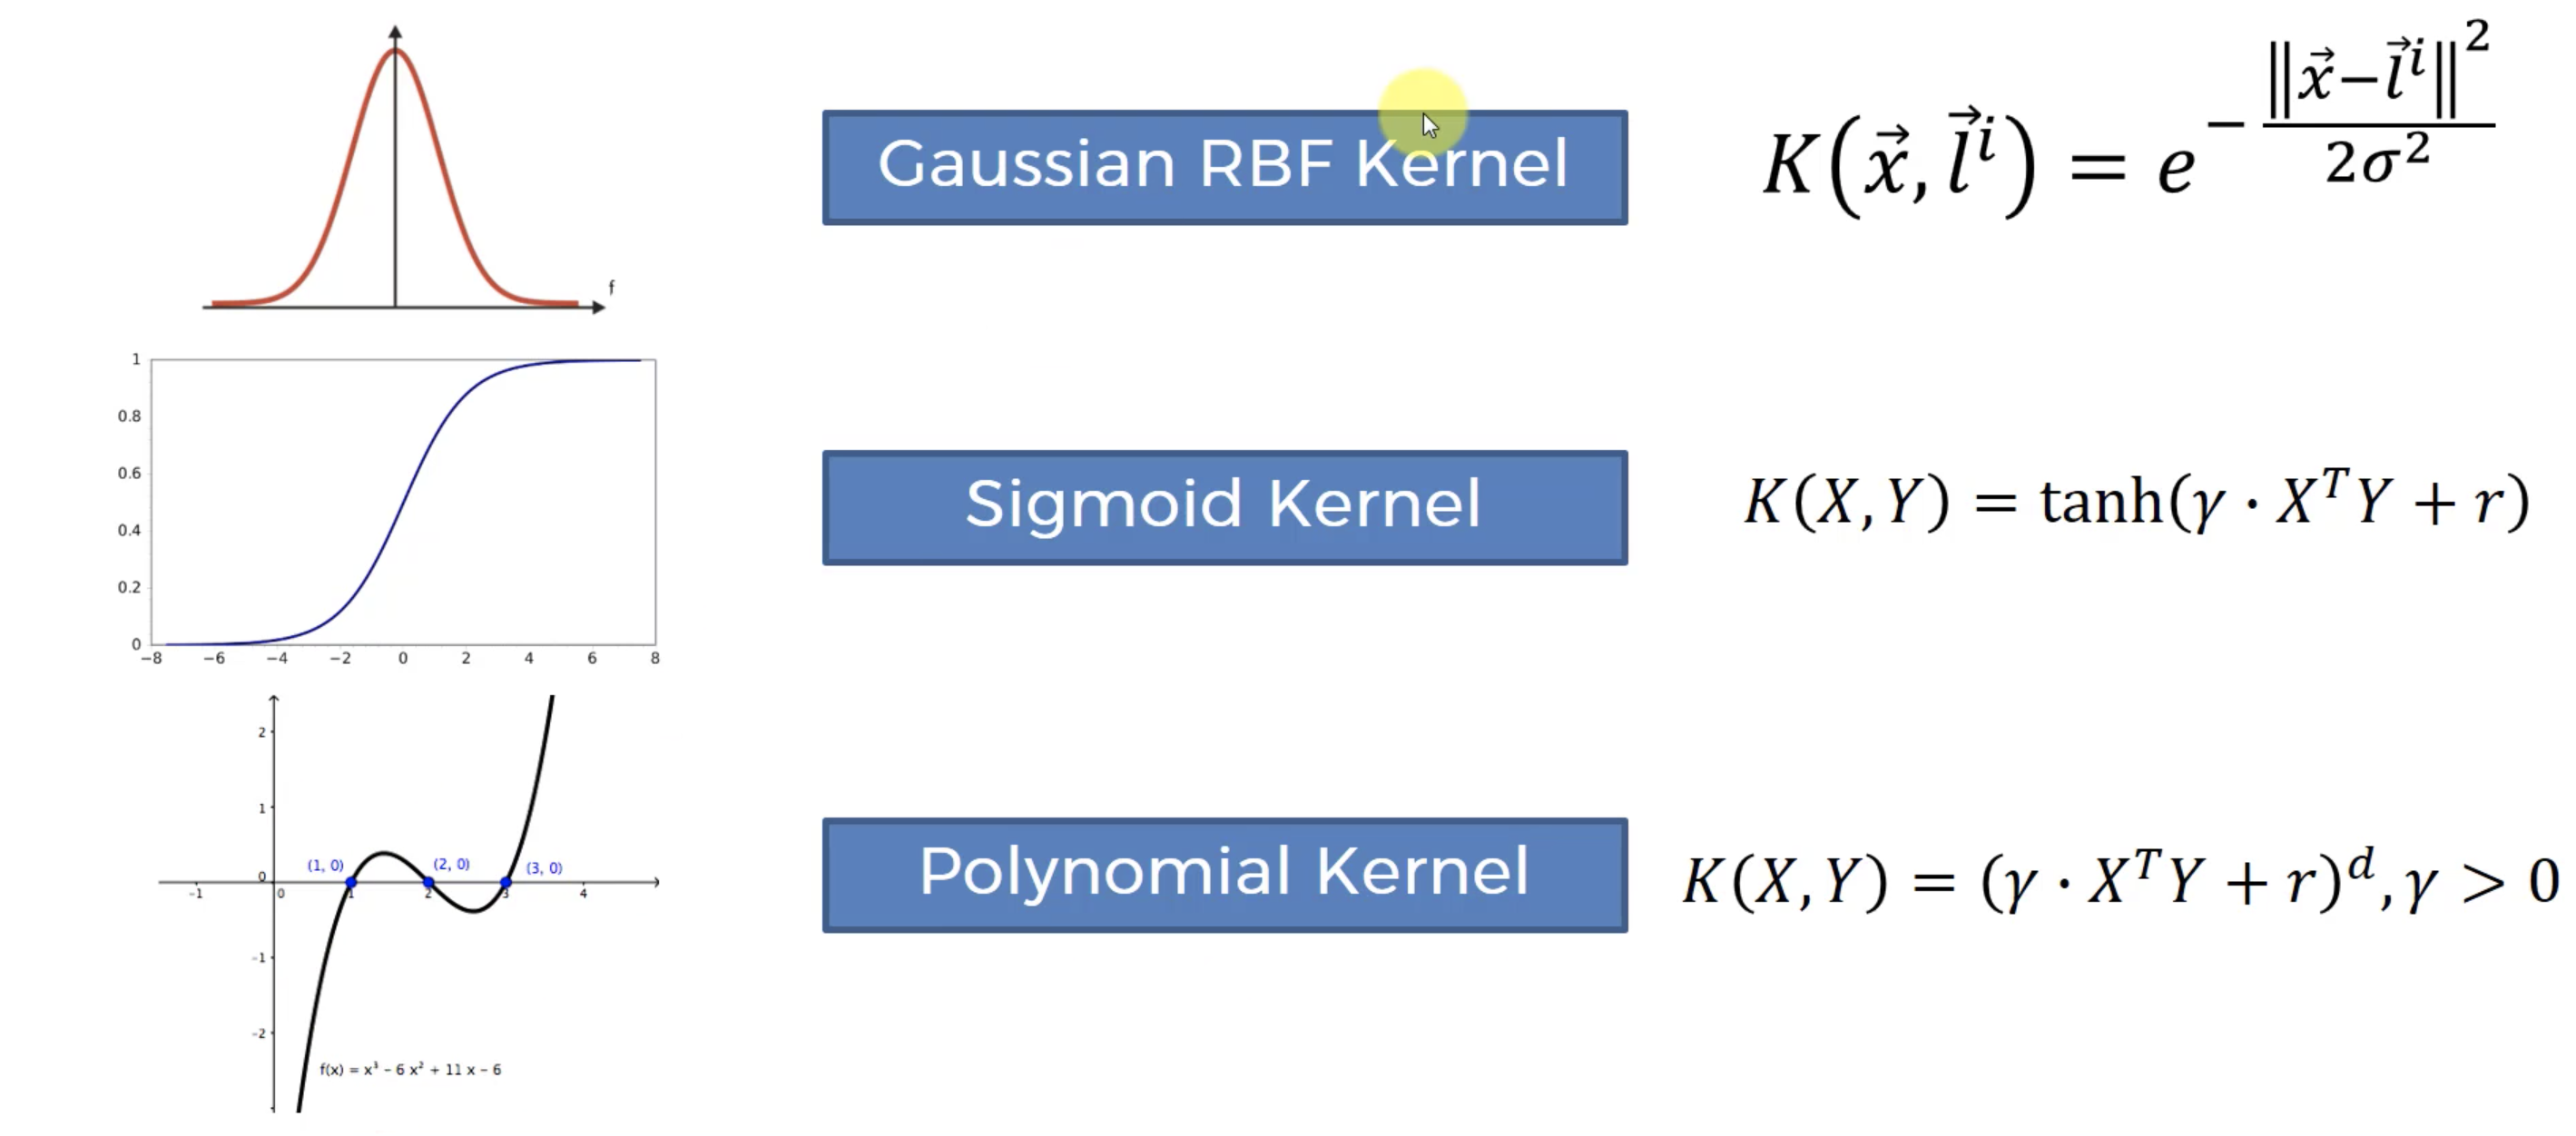
\includegraphics[width=1\linewidth ]{Figures/svm-most-common-kernels.png}

\end{frame}
\end{document}





